\section{EPANET by Example}
\subsection{About}
EPANET is a computer program that performs hydraulics computations in pressure-pipe systems.  
The internal computational engine is similar to that explored in the previous chapter(s), but is far more efficient and well tested.
The current version of EPANET (Official EPA Release) is  2.00.12.  
There is an ongoing Open Source Project that has released a version 2.1 (to follow the release numbering scheme).
There is likely to be a version 2.3 within a few years.  
All the versions so far include a capacity to read an ASCII input file to direct the computations.

A GUI Interface is available that runs in Windows that is quite popular and useful, but it is elderly and newer interfaces are being explored.
Many users dispense with the interface entirely and operate the model using custom-built (or general) wrapper programs to call various DLLs (or Shared Objects).  Wrappers exist in \textbf{R}, Python, Delphi (the Legacy GUI), and probably PERL and Ruby.  

The remainder of this chapter shows how to use EPANET by a series of representative examples.  These examples are at best a subset of the capabilities of the program, but should be enough to get one started.   The program requires some hydraulic insight to interpret the results as well as detect data entry or conceptualization errors.
\footnote{This chapter is from "Cleveland, T.G., Tay, C.C., and Neale, C.N. 2015. EPANET by Example. Department of Civil and Environmental Engineering, Texas Tech University."  available at \\
\url{http://cleveland3.ddns.net/university-courses/ce-3372/3-Readings/EPANETbyExample/}
}
\subsection{Using the Legacy Interface}
\subsubsection{Installing the Program}
The \url{url to install video} shows how to download and install EPANET onto your computer.  
EPANET will run fine on a laptop computer even a Macintosh that has a guest Windows OS (WM-Ware, Parallels, or BootCamp).   

The \url{url to install video} shows how to install an implementation that runs (so-so) on a Macintosh (using a container built using Winebottler and WINE).

The \url{url to install video} shows how to install and run an implementation on a Linux computer (using WINE).

EPANET can also be installed onto a flash-drive and run directly from the drive \footnote{A useful trick on a networked system --- be sure you set up the flash drive to be writeable!  I have never tried this on a non-Windows implementation so cannot comment much on that.}.

\subsection{EPANET Modeling by Example}
EPANET models are comprised of nodes, links,and reservoirs.    Pumps are treated as special links (that add head).  Valves are also treated as special links depending on the valve types.  All models must have a reservoir (or storage tank).

\subsubsection{Defaults}
The program has certain defaults that should be set at the beginning of a simulation.  The main defaults of importance are the head loss equations (Darcy-Weisbach, Hazen-Williams, or Chezy-Manning) and the units (CFS, LPS, etc.)   

\subsubsection{Example 1: Flow in a Single Pipe}
A simple model to consider is a single pipe, a classic problem statement might be something like

\begin{quote}A 5-foot diameter, enamel coated, steel pipe carries 60$^o$F water at a discharge of 295 cubic-feet per second (cfs).  Using the Moody chart, estimate the head loss in a 10,000 foot length of this pipe.
\end{quote}

In EPANET we will start the program, build a tank-pipe system and find the head loss in a 10,000 foot length of the pipe.  The program will compute the friction factor for us (and we can check on the Moody chart if we wish).  


\begin{figure}[htbp] %  figure placement: here, top, bottom, or page
   \centering
   \includegraphics[width=4in]{./23-EPANETbyEXAMPLE/epanet-start.pdf} 
   \caption{Start EPANET program}
   \label{fig:epanet-start}
\end{figure}
The main trick in EPANET is going to be the friction coefficient, in the EPANET manual on page 30 and 31, the author indicates that the program expects a roughness coefficient based on the head loss equation.  The units of the roughness coefficient for a steel pipe are $0.15 \times 10^{-3}$ feet.   On page 71 of the user manual the author states that roughness coefficients are in millifeet (millimeters) when the Darcy-Weisbach head loss model is used.   So keeping that in mind we proceed with the example.

Figure \ref{fig:epanet-start} is a screen capture of the EPANET program after installing the program.   The program starts as a blank slate and we will select a reservoir and a node from the tool bar at the top and place these onto the design canvas.

Figure \ref{fig:epanet-start} is a screen capture of the EPANET program after setting defaults for the simulation.   Failure to set correct units for your problem are sometimes hard to detect (if the model runs), so best to make it a habit to set defaults for all new projects.
\begin{figure}[htbp] %  figure placement: here, top, bottom, or page
   \centering
   \includegraphics[width=4in]{./23-EPANETbyEXAMPLE/set-default.pdf} 
   \caption{Set program defaults.  In this case units are cubic-feet-per-second and loss model is Darcy-Weisbach.}
   \label{fig:set-default}
\end{figure}
Next we add the reservoir and the node.   Figure \ref{fig:place-nodes} is a screen capture after the reservoir and node is placed.
\begin{figure}[htbp] %  figure placement: here, top, bottom, or page
   \centering
   \includegraphics[width=4in]{./23-EPANETbyEXAMPLE/place-nodes.pdf} 
   \caption{Place the reservoir and the demand node.}
   \label{fig:place-nodes}
\end{figure}
We will specify a total head at the reservoir (value is unimportant as long as it is big enough to overcome the head loss and not result in a negative pressure at the node.   We will specify the demand at the node equal to the desired flow in the pipe.     Next we will add the pipe.

\begin{figure}[htbp] %  figure placement: here, top, bottom, or page
   \centering
   \includegraphics[width=5in]{./23-EPANETbyEXAMPLE/add-link.pdf} 
   \caption{Link the reservoir and demand node with a pipe.}
   \label{fig:add-link}
\end{figure}

Figure \ref{fig:add-link} is a screen capture after the pipe is placed.  The sense of flow in this example is from reservoir to node, but if we had it backwards we could either accept a negative flow in the pipe, or right-click the pipe and reverse the start and end node connections.

\newpage
Now we can go back to each hydraulic element in the model and edit the properties.  We supply pipe properties (diameter, length, roughness height) as in Figure \ref{fig:link-properties}.
\begin{figure}[h!] %  figure placement: here, top, bottom, or page
   \centering
   \includegraphics[width=4in]{./23-EPANETbyEXAMPLE/link-properties.pdf} 
   \caption{Set the pipe length, diameter, and roughness height.}
   \label{fig:link-properties}
\end{figure}
We supply the reservoir total head as in Figure \ref{fig:set-head}.
\begin{figure}[htbp] %  figure placement: here, top, bottom, or page
   \centering
   \includegraphics[width=4in]{./23-EPANETbyEXAMPLE/set-head.pdf} 
   \caption{Set the reservoir total head, 100 feet should be enough in this example.}
   \label{fig:set-head}
\end{figure}
\clearpage
We set the demand node elevation and the actual desired flow rate as in Figure \ref{fig:set-demand}.
\begin{figure}[htbp] %  figure placement: here, top, bottom, or page
   \centering
   \includegraphics[width=4in]{./23-EPANETbyEXAMPLE/set-demand.pdf} 
   \caption{Set the node elevation and demand.  In this case the elevation is set to zero (the datum) and the demand is set to 295 cfs as per the problem statement.}
   \label{fig:set-demand}
\end{figure}
The program is now ready to run, next step would be to save the input file (File/Save/Name), then run the program by selecting the lighting bolt looking thing and the computation engine will start.  

\begin{figure}[htbp] %  figure placement: here, top, bottom, or page
   \centering
   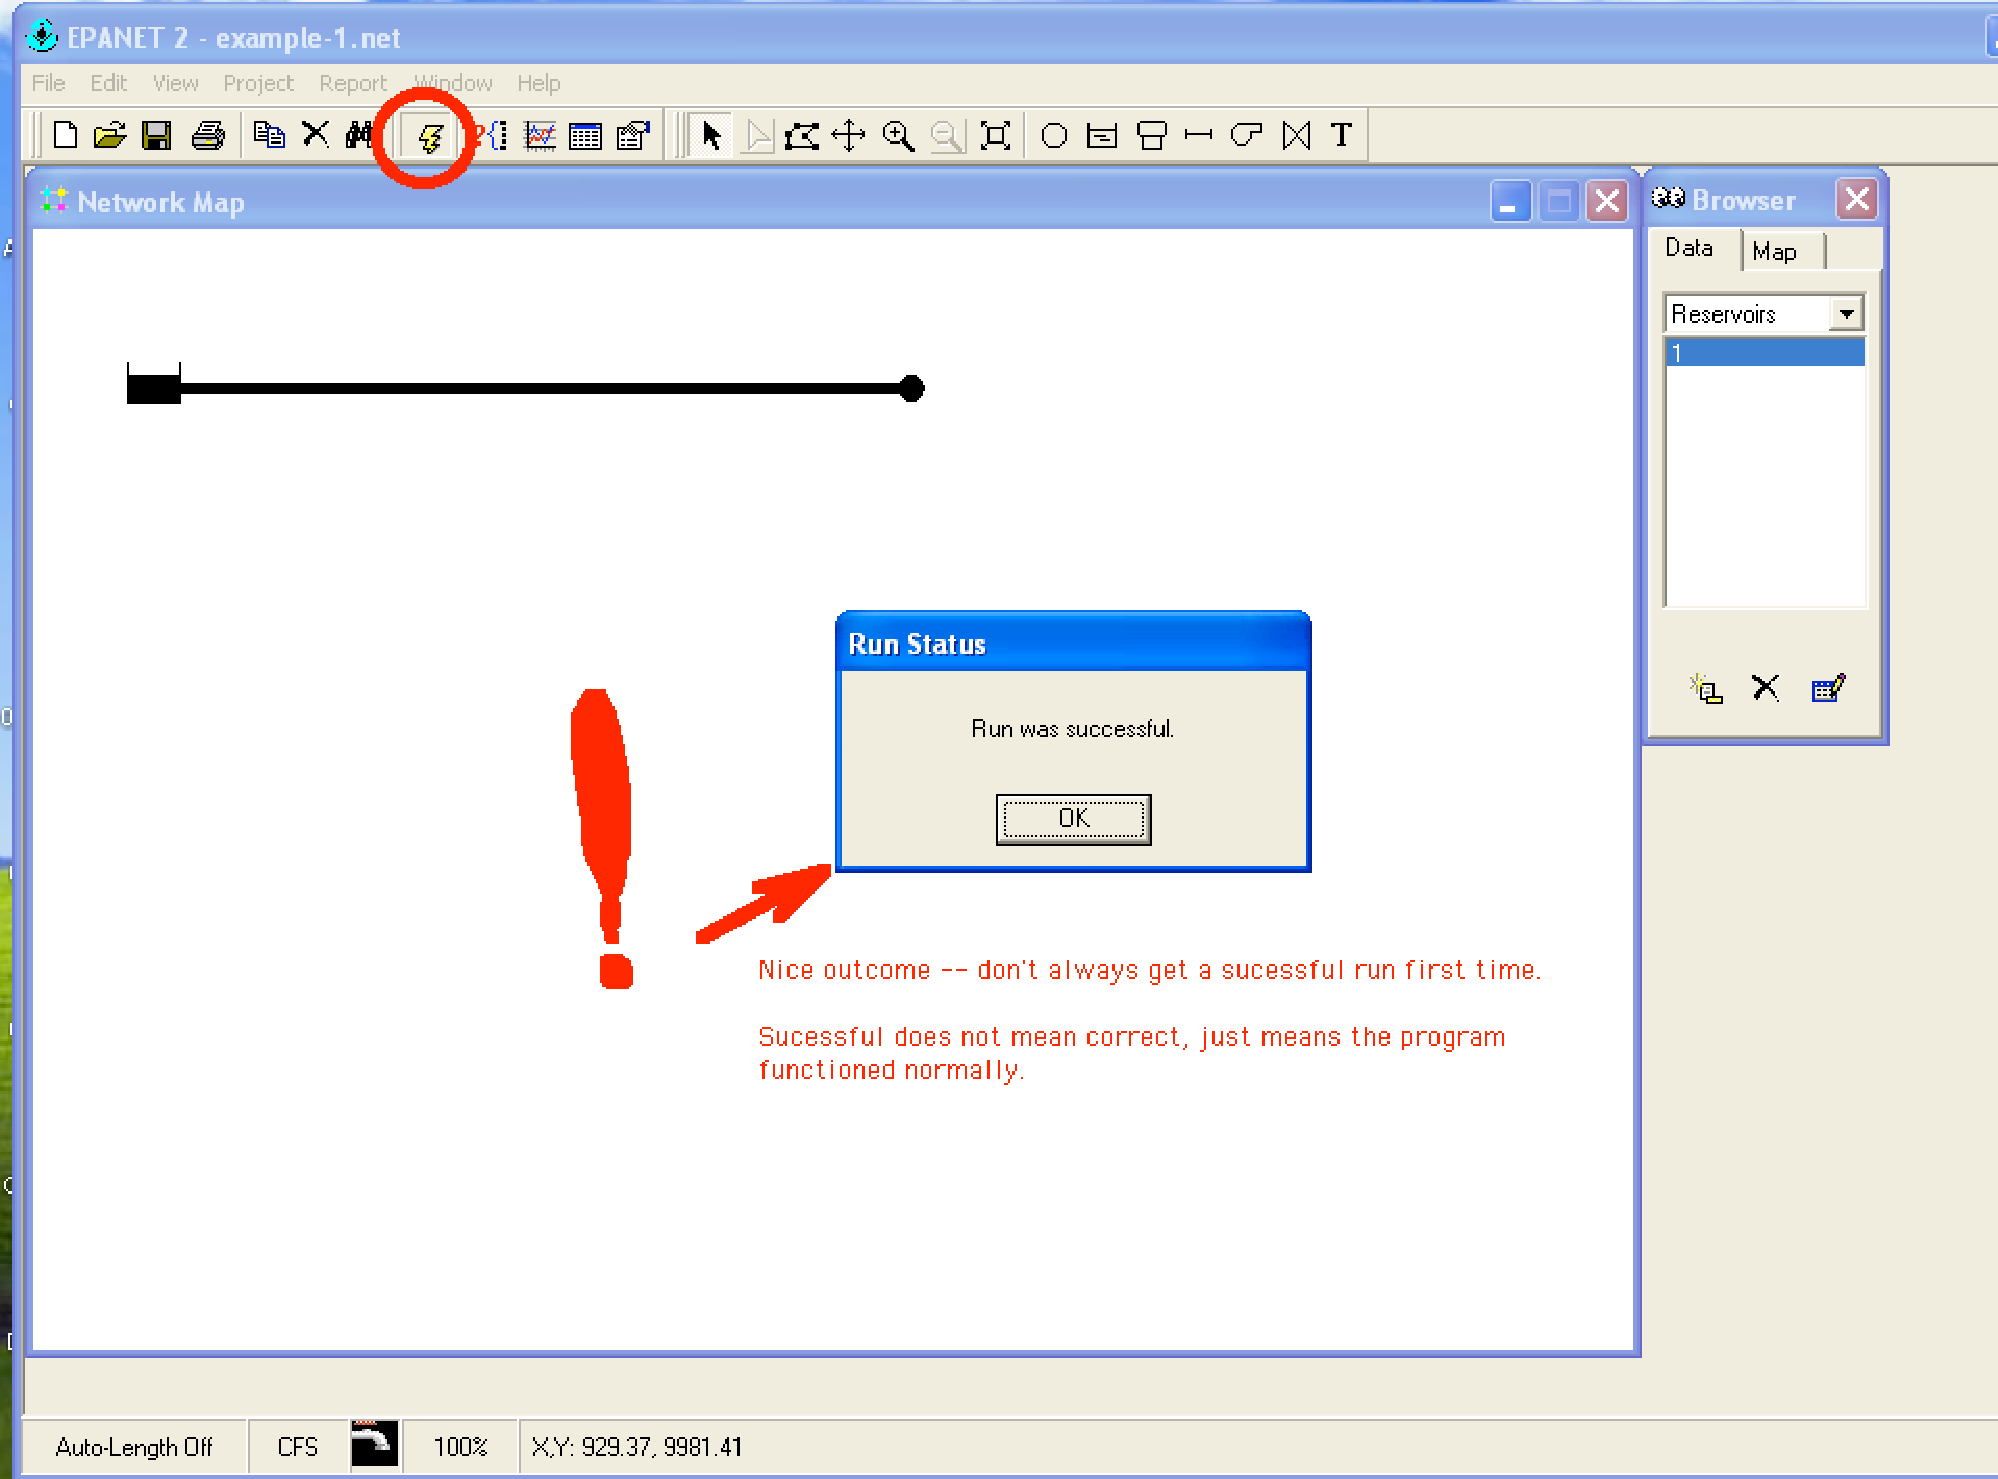
\includegraphics[width=3.5in]{./23-EPANETbyEXAMPLE/run-program.pdf} 
   \caption{Running the program}
   \label{fig:run-program}
\end{figure}

If the nodal connectivity is OK and there are no computed negative pressures the program will run.   Figure \ref{fig:run-program}  is the appearance of the program after the run is complete (the annotations are mine!).
A successful run means the program found an answer to the problem you provided -- whether it is the correct answer to your problem requires the engineer to interpret results and decide if they make sense.  The more common conceptualization errors are incorrect units and head loss equation for the supplied roughness values, missed connections, and forgetting demand somewhere.  With practice these kind of errors are straightforward to detect.   In the present example we select the pipe and the solution values are reported at the bottom of a dialog box.


\begin{figure}[htbp] %  figure placement: here, top, bottom, or page
   \centering
   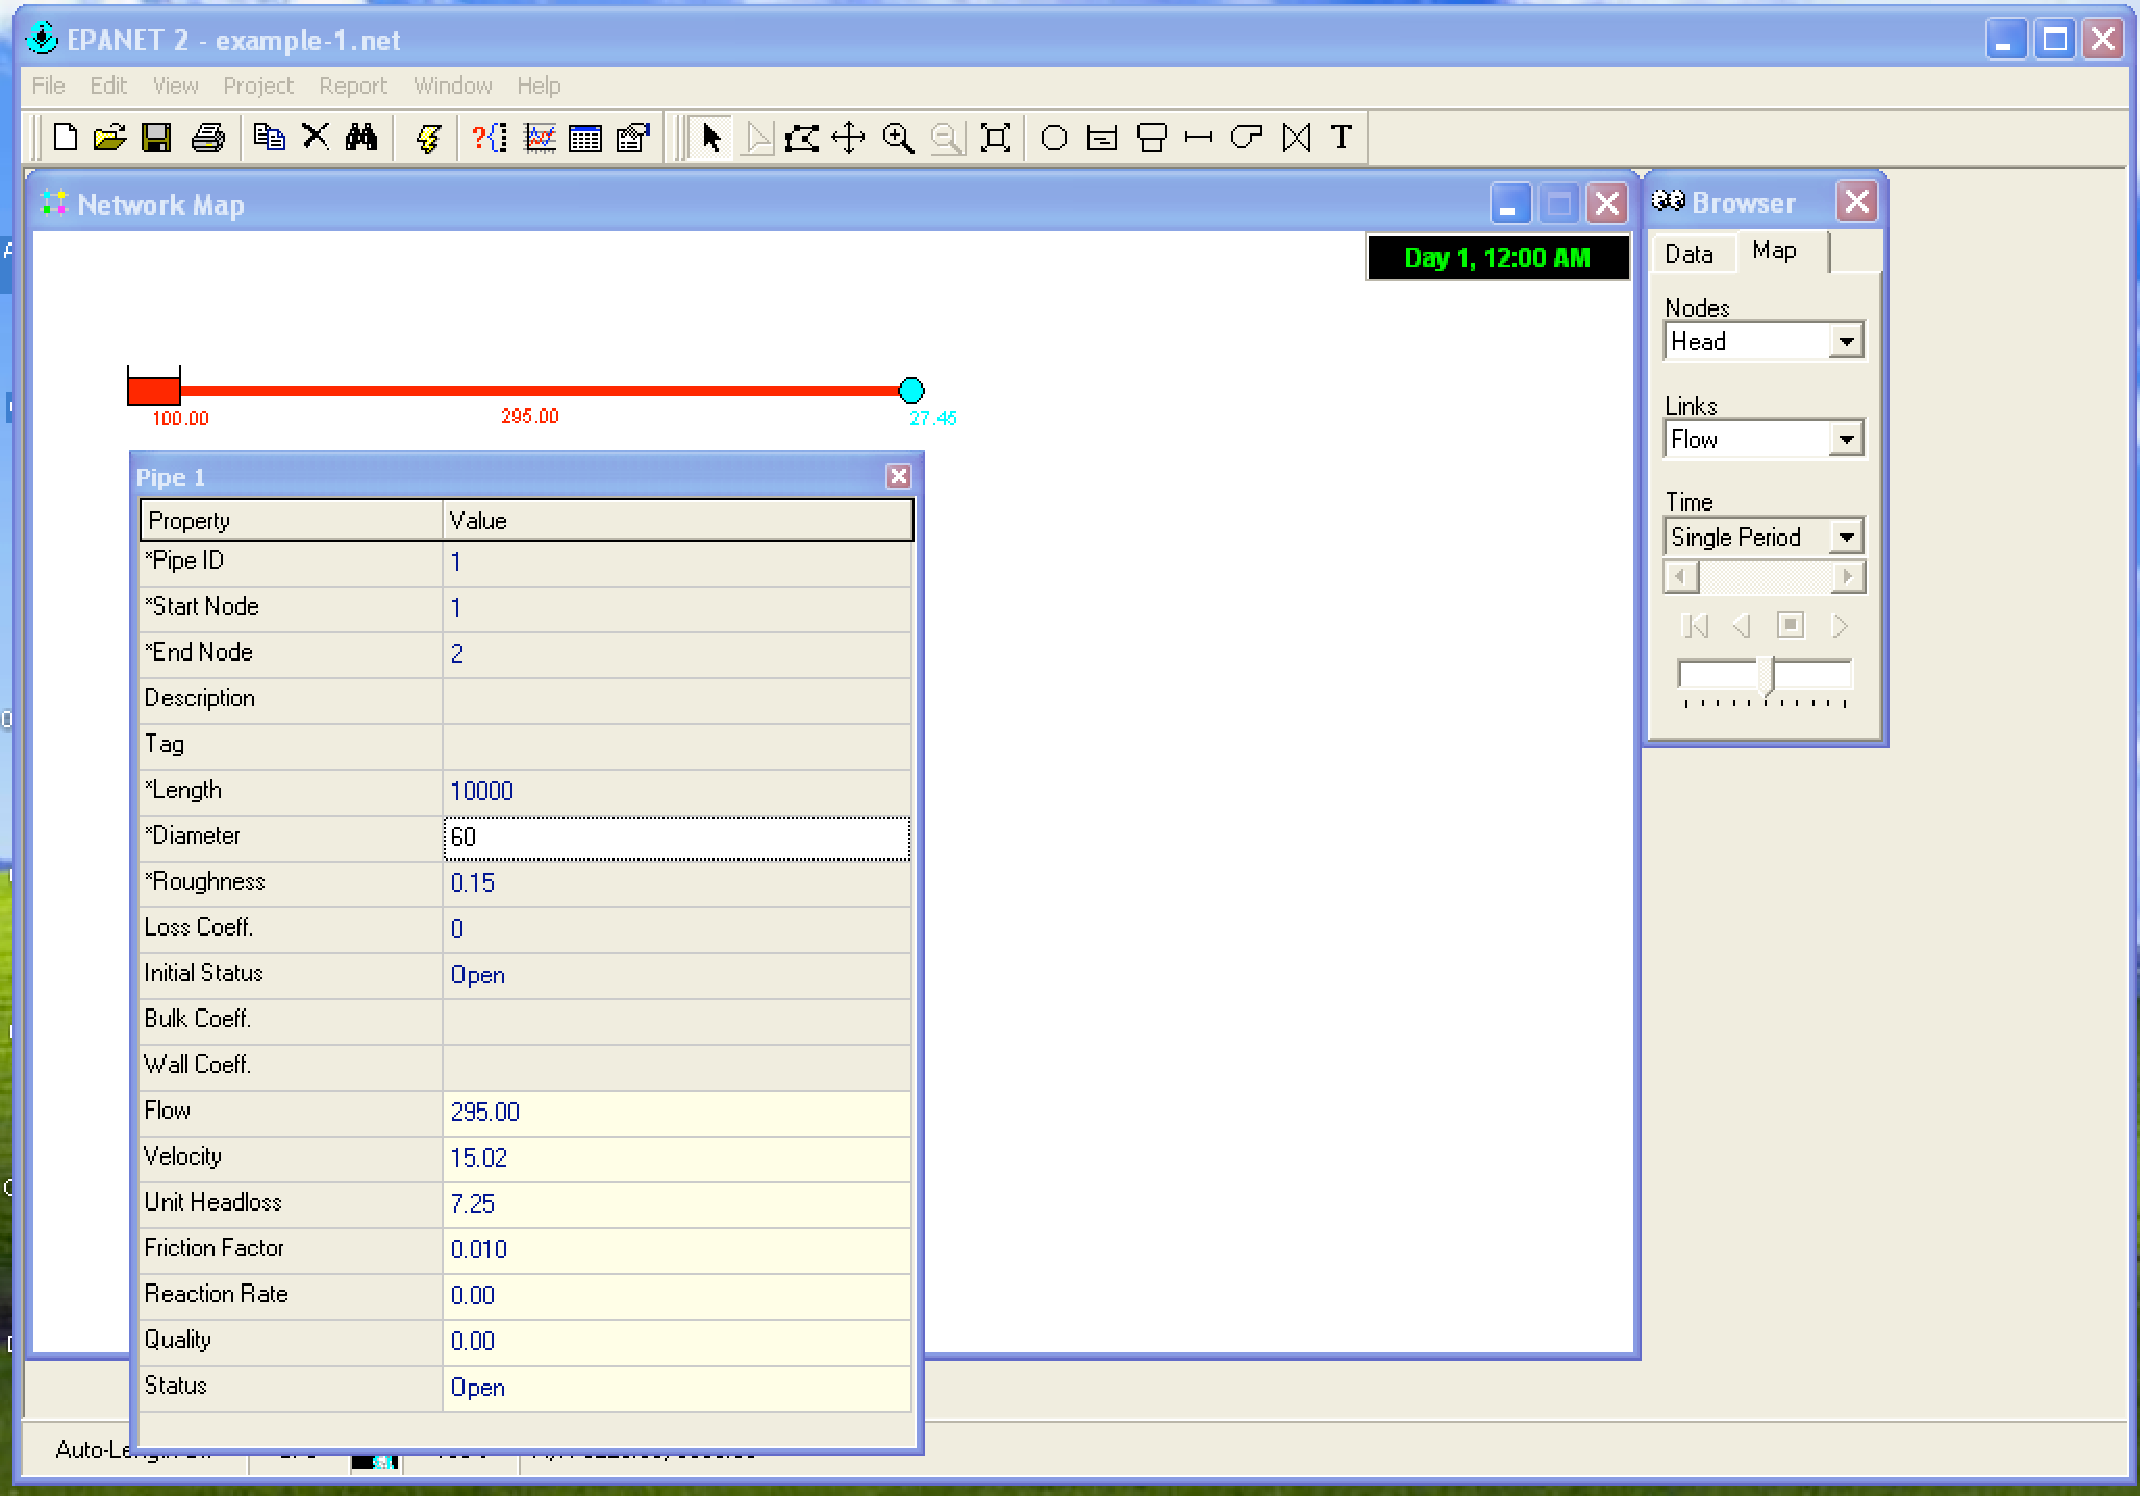
\includegraphics[width=4in]{./23-EPANETbyEXAMPLE/interpret-solution.pdf} 
   \caption{Solution dialog box for the pipe.}
   \label{fig:interpret-solution}
\end{figure}

Figure \ref{fig:interpret-solution} is the result of turning on the computed head values at the node (and reservoir) and the flow value for the pipe.  The dialog box reports about 7.2 feet of head loss per 1000 feet of pipe for a total of 72 feet of head loss in the system.   The total head at the demnad node is about 28 feet, so the head loss plus remaining head at the node is equal to the 100 feet of head at the reservoir, the anticipated result.  

The computed friction factor is 0.010, which we could check against the Moody chart if we wished to adjust the model to agree with some other known friction factor.   
\clearpage
%%%%%%%%%%%%%%%%%%%%%%%%%%
%%%%%%%%%%%%%%%%%%%%%%%%%%%%%%%%%
%%%%%%%%%%%%%%%%%%%%%%%%%%%%%%%%%%%%%%%%
\subsubsection{Example 2: Flow Between Two Reservoirs}
This example represents the situation where the total head is known at two points on a pipeline, and one wishes to determine the flow rate (or specify a flow rate and solve for a pipe diameter).   Like the prior example it is contrived, but follows the same general modeling process.

As in the prior example, we will use EPANET to solve a problem we have already solved by hand.

\begin{quote}
Using the Moody chart, and the energy equation, estimate the diameter of a cast-iron pipe needed to carry 60$^o$F water at a discharge of 10 cubic-feet per second (cfs) between two reservoirs 2 miles apart.  The elevation difference between the water surfaces in the two reservoirs is 20 feet.
\end{quote}

As in the prior example, we will need to specify the pipe roughness terms, then solve by trial-and-error for the diameter required to carry the water at the desired flowrate.  Page 31 of the EPANET manual suggests that the roughness height for cast iron is 0.85 millifeet.  

As before the steps to model the situation are:
\begin{enumerate}
\item Start EPANET
\item Set defaults
\item Select the reservoir tool.  Put two reservoirs on the map.
\item Select the node tool, put a node on the map. \textbf{EPA NET needs one node!}
\item Select the link (pipe) tool, connect the two reservoirs to the node.  One link is the 2 mile pipe, the other is a short large diameter pipe (negligible head loss).
\item Set the total head each reservoir.
\item Set the pipe length and roughness height in the 2 mile pipe.
\item Guess a diameter.
\item Save the input file.
\item Run the program.   Query the pipe and find the computed flow.  If the flow is too large reduce the pipe diameter, if too small increase the pipe diameter.  Stop when within a few percent of the desired flow rate.  Use commercially available diameters in the trial-and-error process, so exact match is not anticipated.
\end{enumerate}

Figure \ref{fig:new-solution} is a screen capture after the model is built and some trial-and-error diameter selection.   Of importance is the node and the ``short pipe'' that connects the second reservoir.   By changing the diameter (inches) in the dialog box and re-running the program we can find a solution (diameter) that produces 10 cfs in the system for the given elevation differences.  

\begin{figure}[htbp] %  figure placement: here, top, bottom, or page
   \centering
   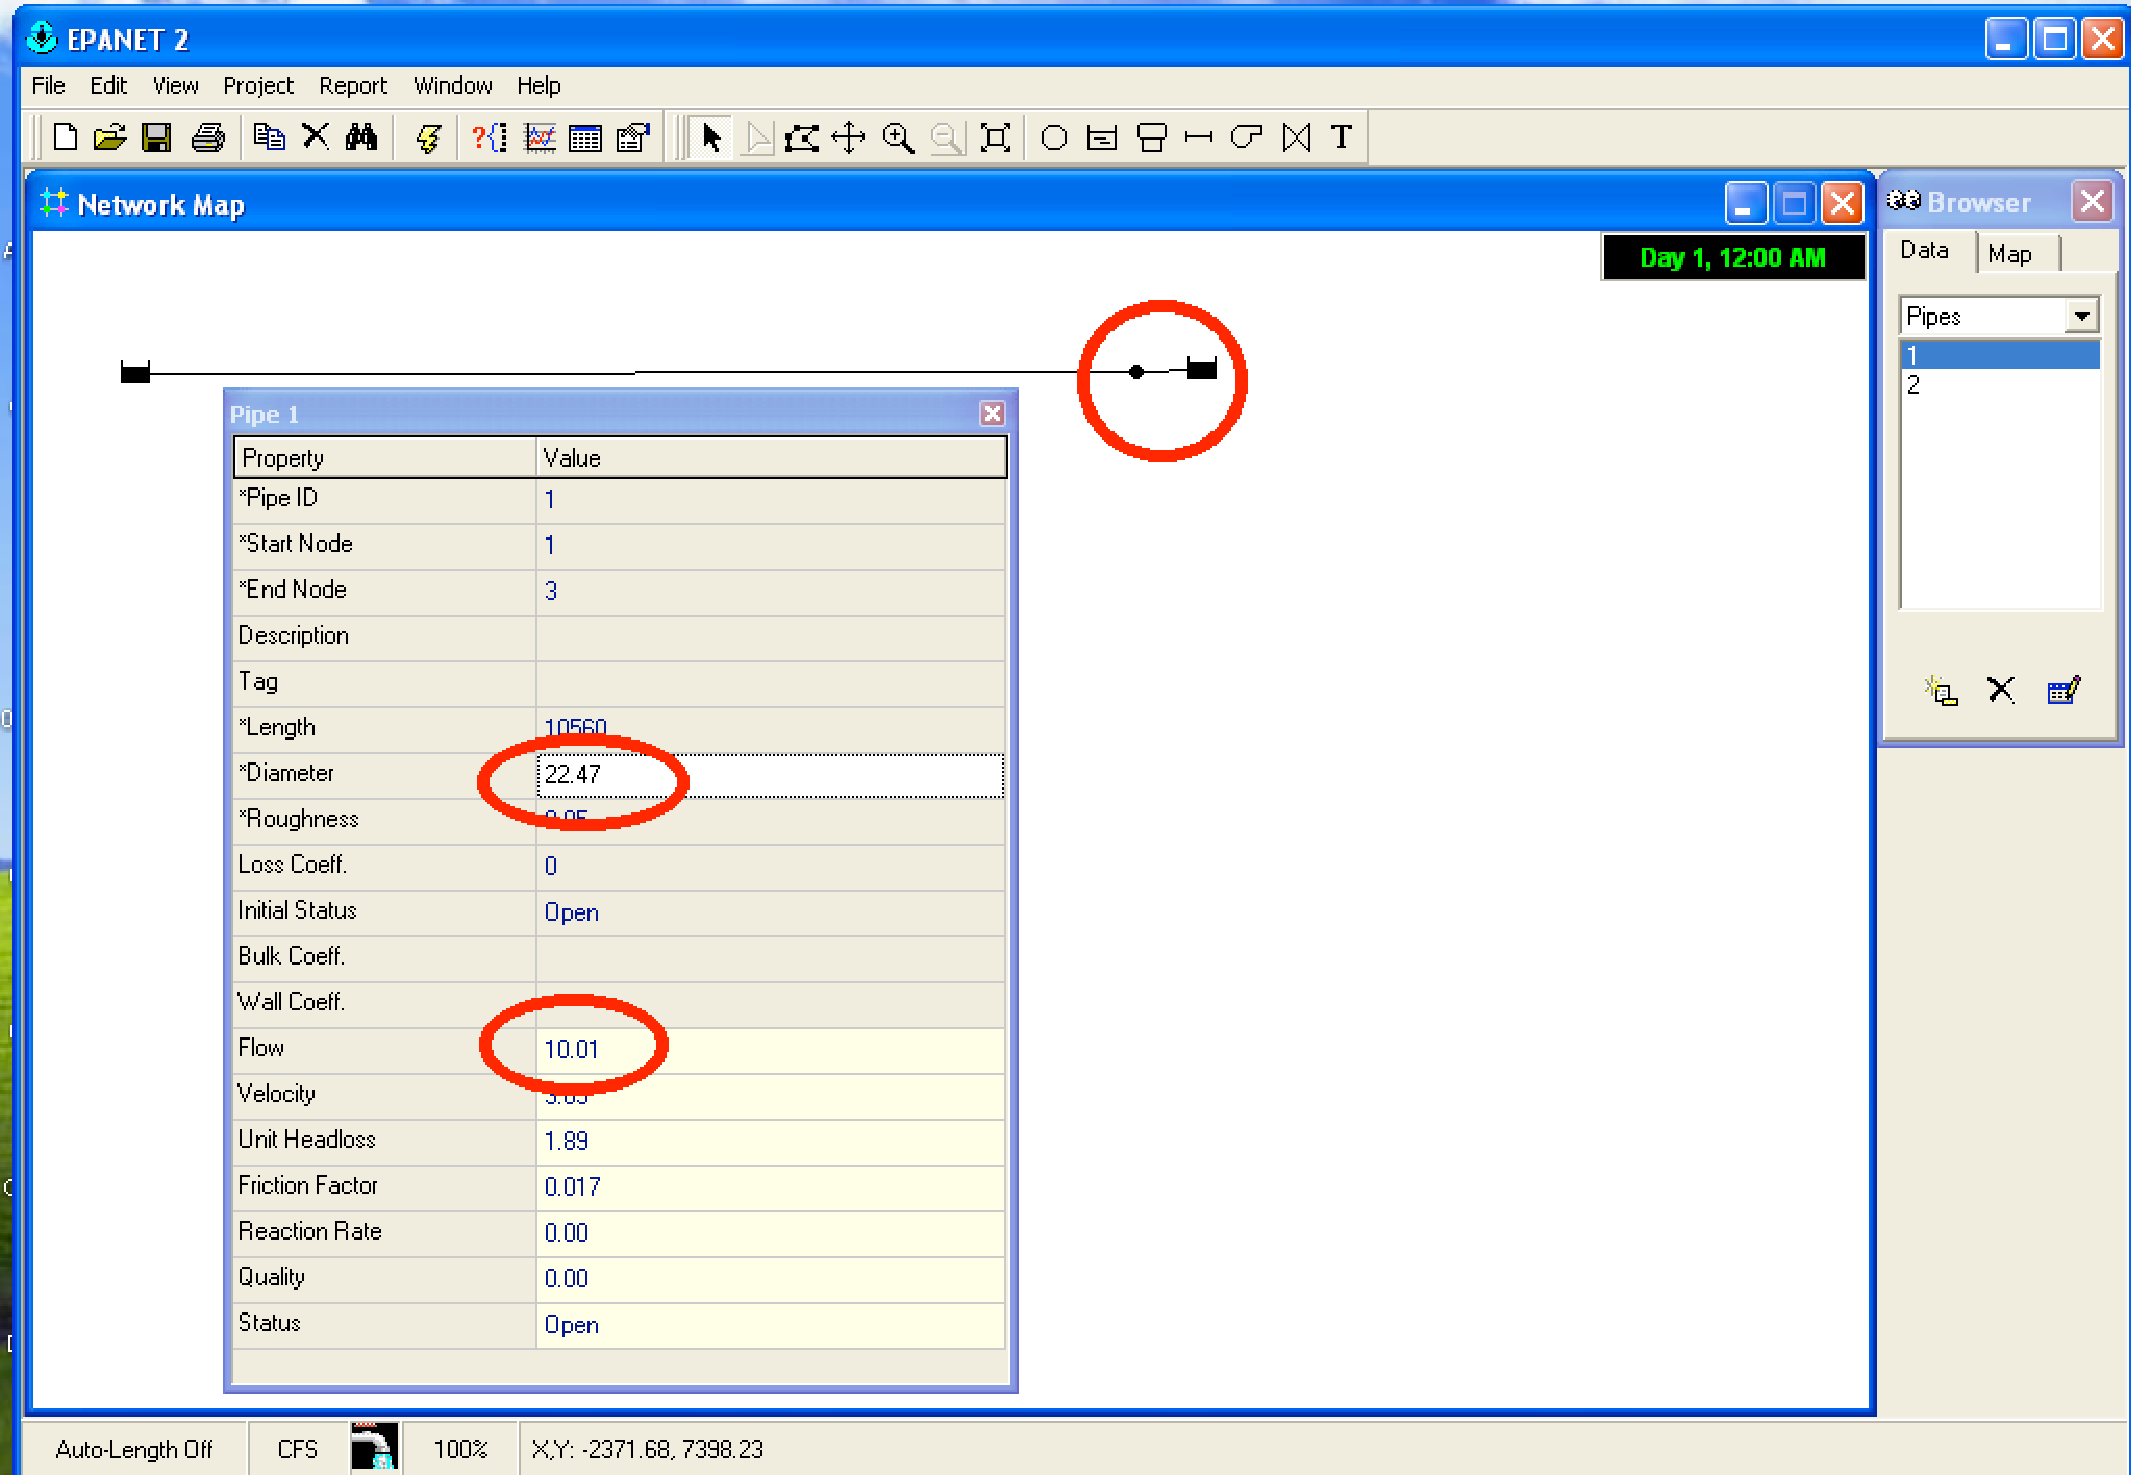
\includegraphics[width=6in]{./23-EPANETbyEXAMPLE/new-solution.pdf} 
   \caption{Solution dialog box for the pipe for Example 2}
   \label{fig:new-solution}
\end{figure}

We would conclude from this use of EPANET that a 22.75 inch ID cast iron pipe would convey 10 cfs between the two reservoirs.  Compare this solution to the ``by-hand'' soluton to see if they are close.
\clearpage
\subsubsection{Example 3: Three-Reservoir-Problem}
This example repeats another prior problem, but introduces the concept of a basemap (image) to help draw the network.  First the problem statement

\begin{quote}
Reservoirs A, B, and C are connected as shown\footnote{This problem is identical to Chin Problem 2.30, Pg. 92} in Figure \ref{fig:p230}.  The water elevations in reservoirs A, B, and C are 100 m, 80 m, and 60 m.   The three pipes connecting the reservoirs meet at junction J, with pipe AJ being 900 m long, BJ being 800 m long, and CJ being 700 m long.  The diameters of all the pipes are
850 mm.  If all the pipes are ductile iron, and the water temperature is 293$^o$K, find the direction and magnitude of flow in each pipe.

\begin{figure}[htbp] %  figure placement: here, top, bottom, or page
   \centering
   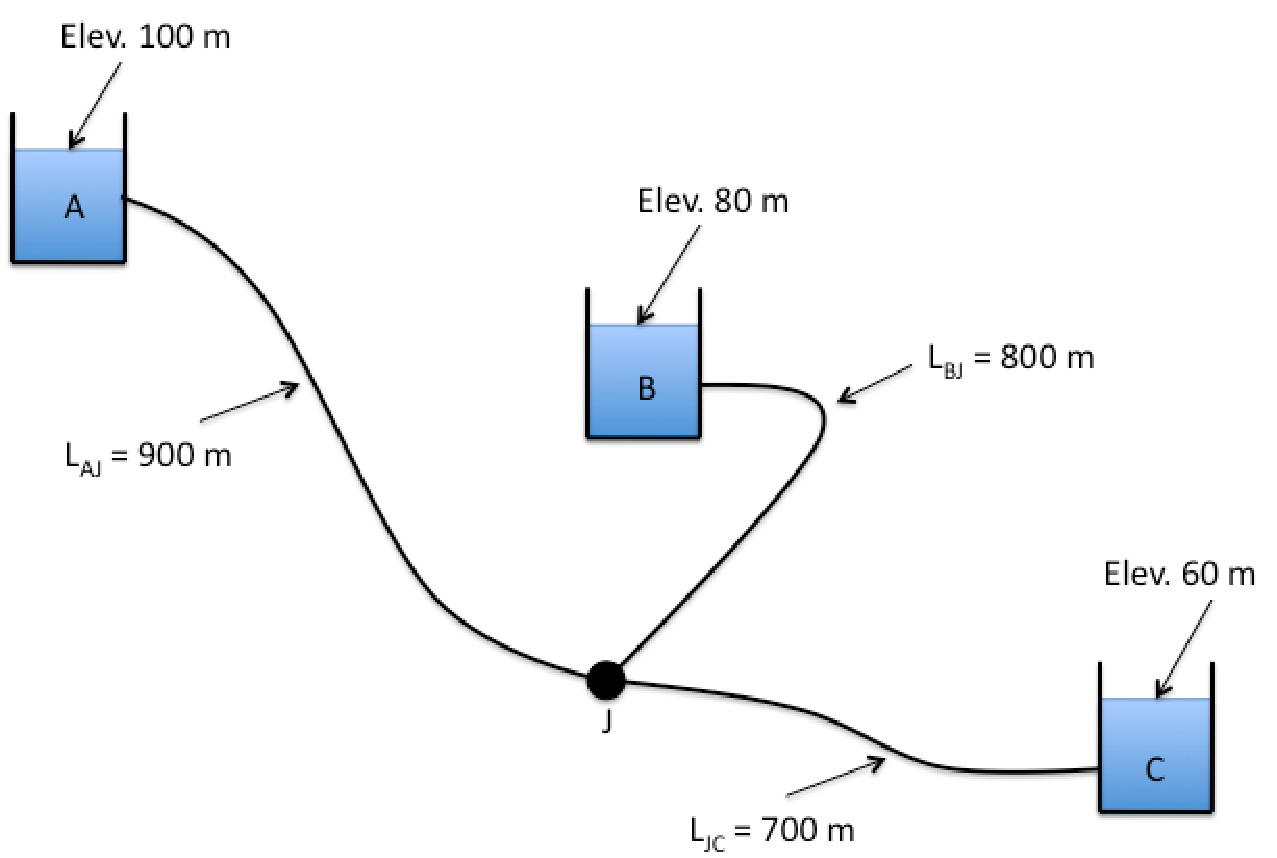
\includegraphics[width=5in]{./23-EPANETbyEXAMPLE/p230.pdf} 
   \caption{Three-Reservoir System Schematic}
   \label{fig:p230}
\end{figure}
\end{quote}

Here we will first convert the image into a bitmap (.bmp) file so EPANET can import the background image and we can use it to help draw the network.  The remainder of the problem is reasonably simple and is an extension of the previous problem.

The steps to model the situation are:
\begin{enumerate}
\item Convert the image into a bitmap, place the bitmap into a directory where the model input file will be stored.
\item Start EPANET
\item Set defaults
\item Import the background.
\item Select the reservoir tool.  Put three reservoirs on the map.
\item Select the node tool, put the node on the map.
\item Select the link (pipe) tool, connect the three reservoirs to the node.  
\item Set the total head each reservoir.
\item Set the pipe length, roughness height, and diameter in each pipe.
\item Save the input file.
\item Run the program.   
\end{enumerate}

Figure \ref{fig:3reservoir-epanet} is the result of the above steps.   In this case the default units were changed to LPS (liters per second).  The roughness height is about 0.26 millimeters (if converted from the 0.85 millifeet unit).

\begin{figure}[htbp] %  figure placement: here, top, bottom, or page
   \centering
   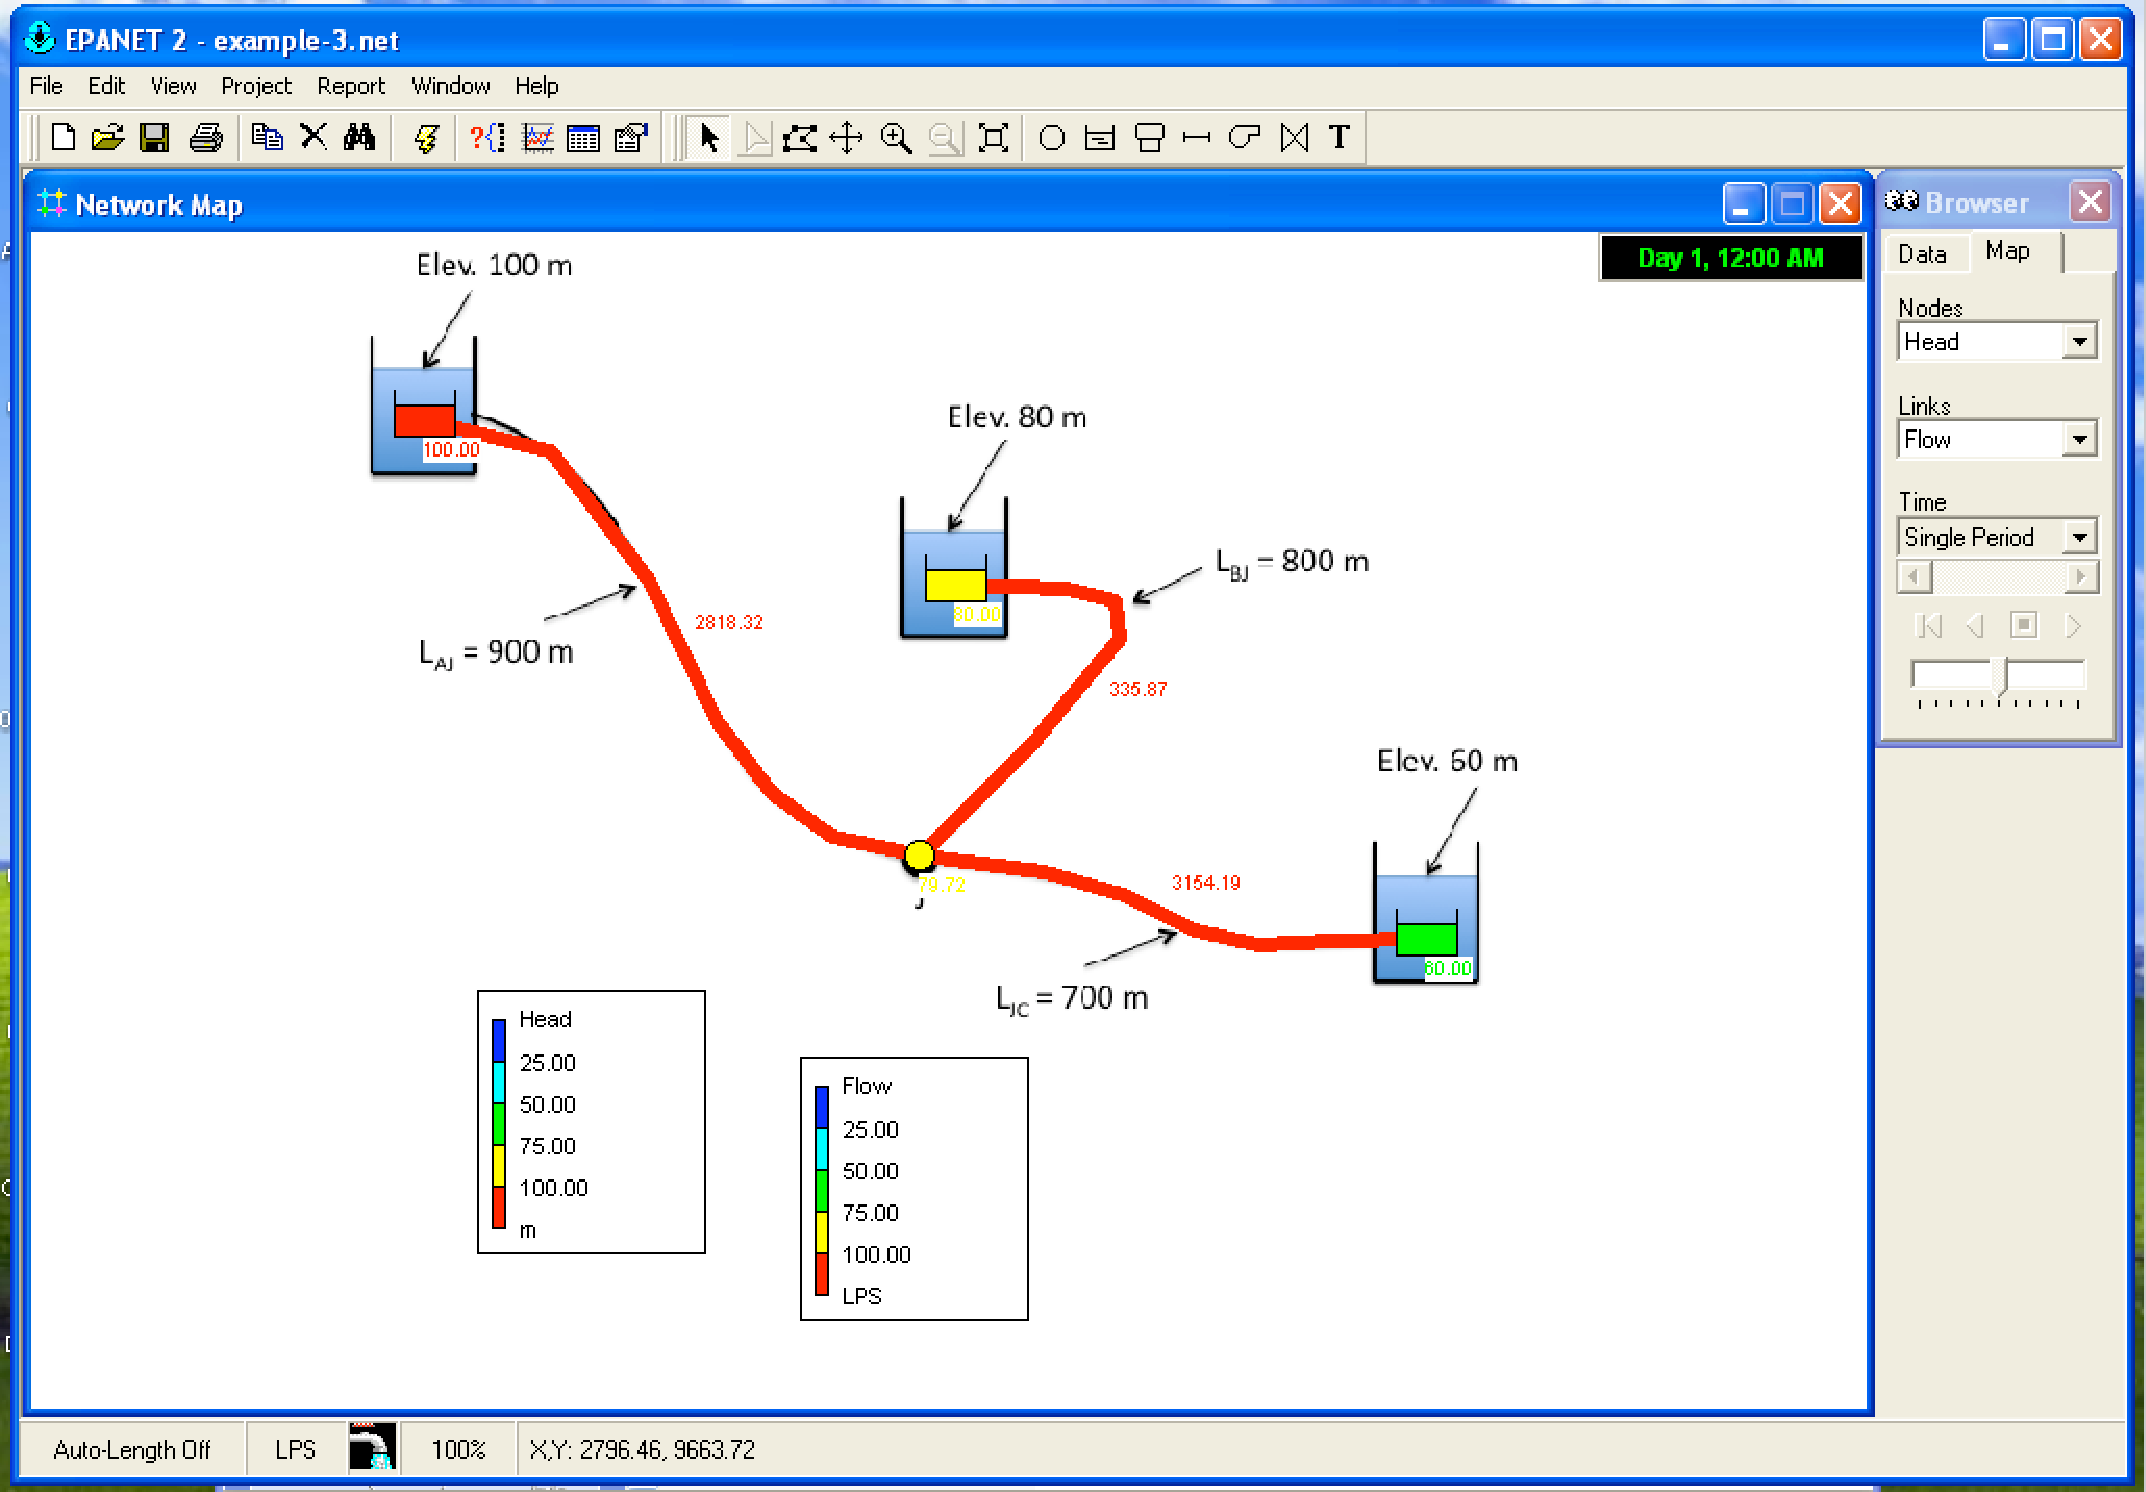
\includegraphics[width=6in]{./23-EPANETbyEXAMPLE/3reservoir-epanet.pdf} 
   \caption{Solution for Example 3.  The pipes were originally straight segments, but a drawing tool in EPANET is used to follow the shape of the underlying basemap.   The training video shows the pipes as the straight lines.  The flowrates are in liters-per-second, divide by 1000 to obtain cubic-meters-per-second.}
   \label{fig:3reservoir-epanet}
\end{figure}
\clearpage
%%%%%%%%%%%%%%%%%%%%%%%%%%%%%%%%%%%%%%%%
\subsubsection{Example 4: A Simple Network}
Expanding the examples, we will next consider a looped network.   As before we will use a prior exercise as the motivating example.

\begin{quote}
The water-supply network shown in Figure \ref{fig:p231} has constant-head elevated storage tanks at A and C, with inflow and outflow at B and D.  The network is on flat terrain with node elevations all equal to 50 meters\footnote{This problem is similar to Chin Problem 2.31, Pg. 92}.  If all pipes are ductile iron, compute the inflows/outflows to the storage tanks.   Assume that flow in all pipes are fully turbulent.

\begin{figure}[htbp] %  figure placement: here, top, bottom, or page
   \centering
   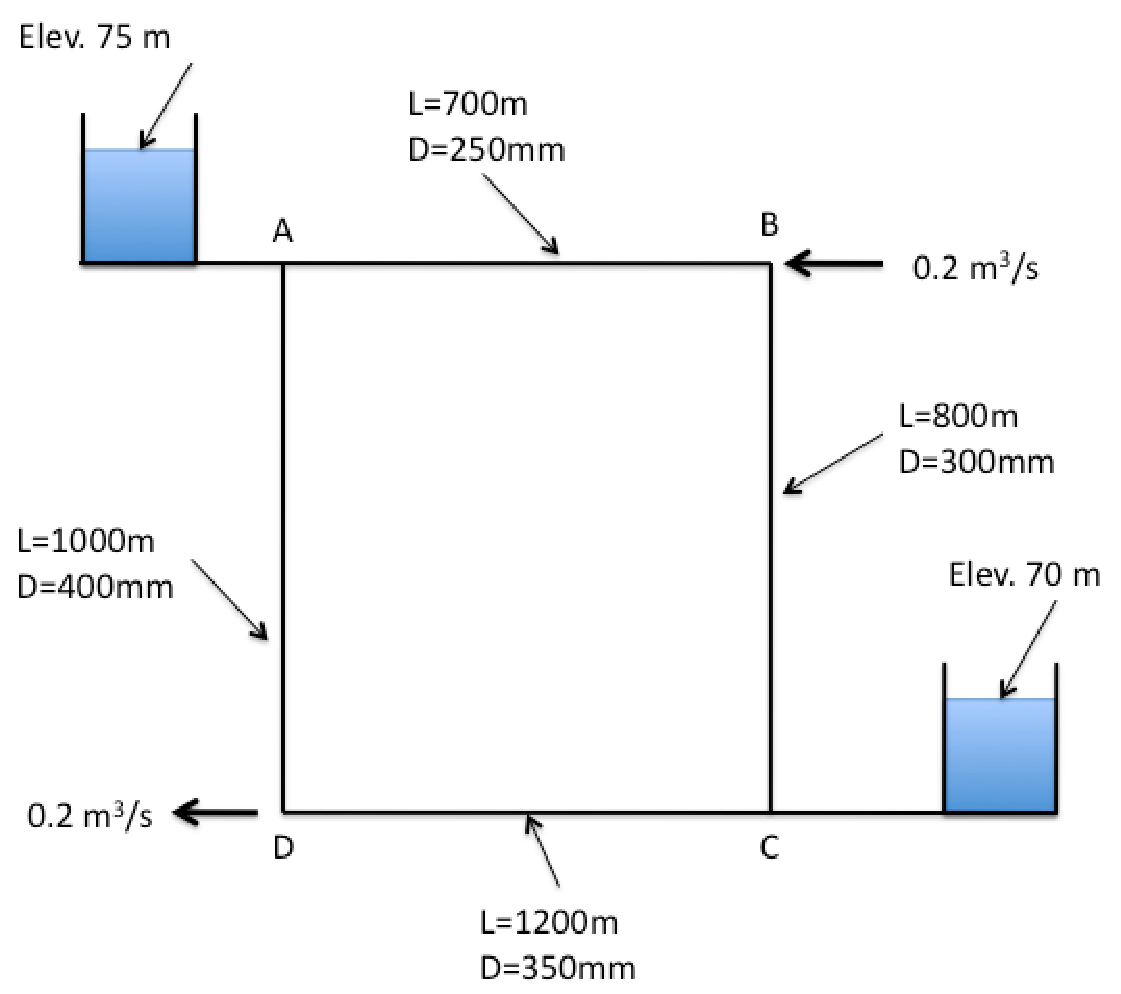
\includegraphics[width=5in]{./23-EPANETbyEXAMPLE/p231.pdf} 
   \caption{Two-Tank Distribution System Schematic}
   \label{fig:p231}
\end{figure}
\end{quote}

As before we will follow the modeling protocol but add demand at the nodes.

The steps to model the situation are:
\begin{enumerate}
\item Convert the image into a bitmap, place the bitmap into a directory where the model input file will be stored.
\item Start EPANET
\item Set defaults
\item Import the background.
\item Select the reservoir tool.  Put two reservoirs on the map.
\item Select the node tool, put 4 nodes on the map.
\item Select the link (pipe) tool, connect the reservoirs to their nearest nodes.  Connect the nodes to each other.  
\item Set the total head each reservoir.
\item Set the pipe length, roughness height, and diameter in each pipe.  The pipes that connect to the reservoirs should be set as short and large diameter, we want negligible head loss in these pipes so that the reservoir head represents the node heads at these locations.
\item Save the input file.
\item Run the program.   
\end{enumerate}

In this case the key issues are the units (liters per second) and roughness height (0.26 millimeters).   Figure \ref{fig:simple-network} is a screen capture of a completed model.   

\begin{figure}[htbp] %  figure placement: here, top, bottom, or page
   \centering
   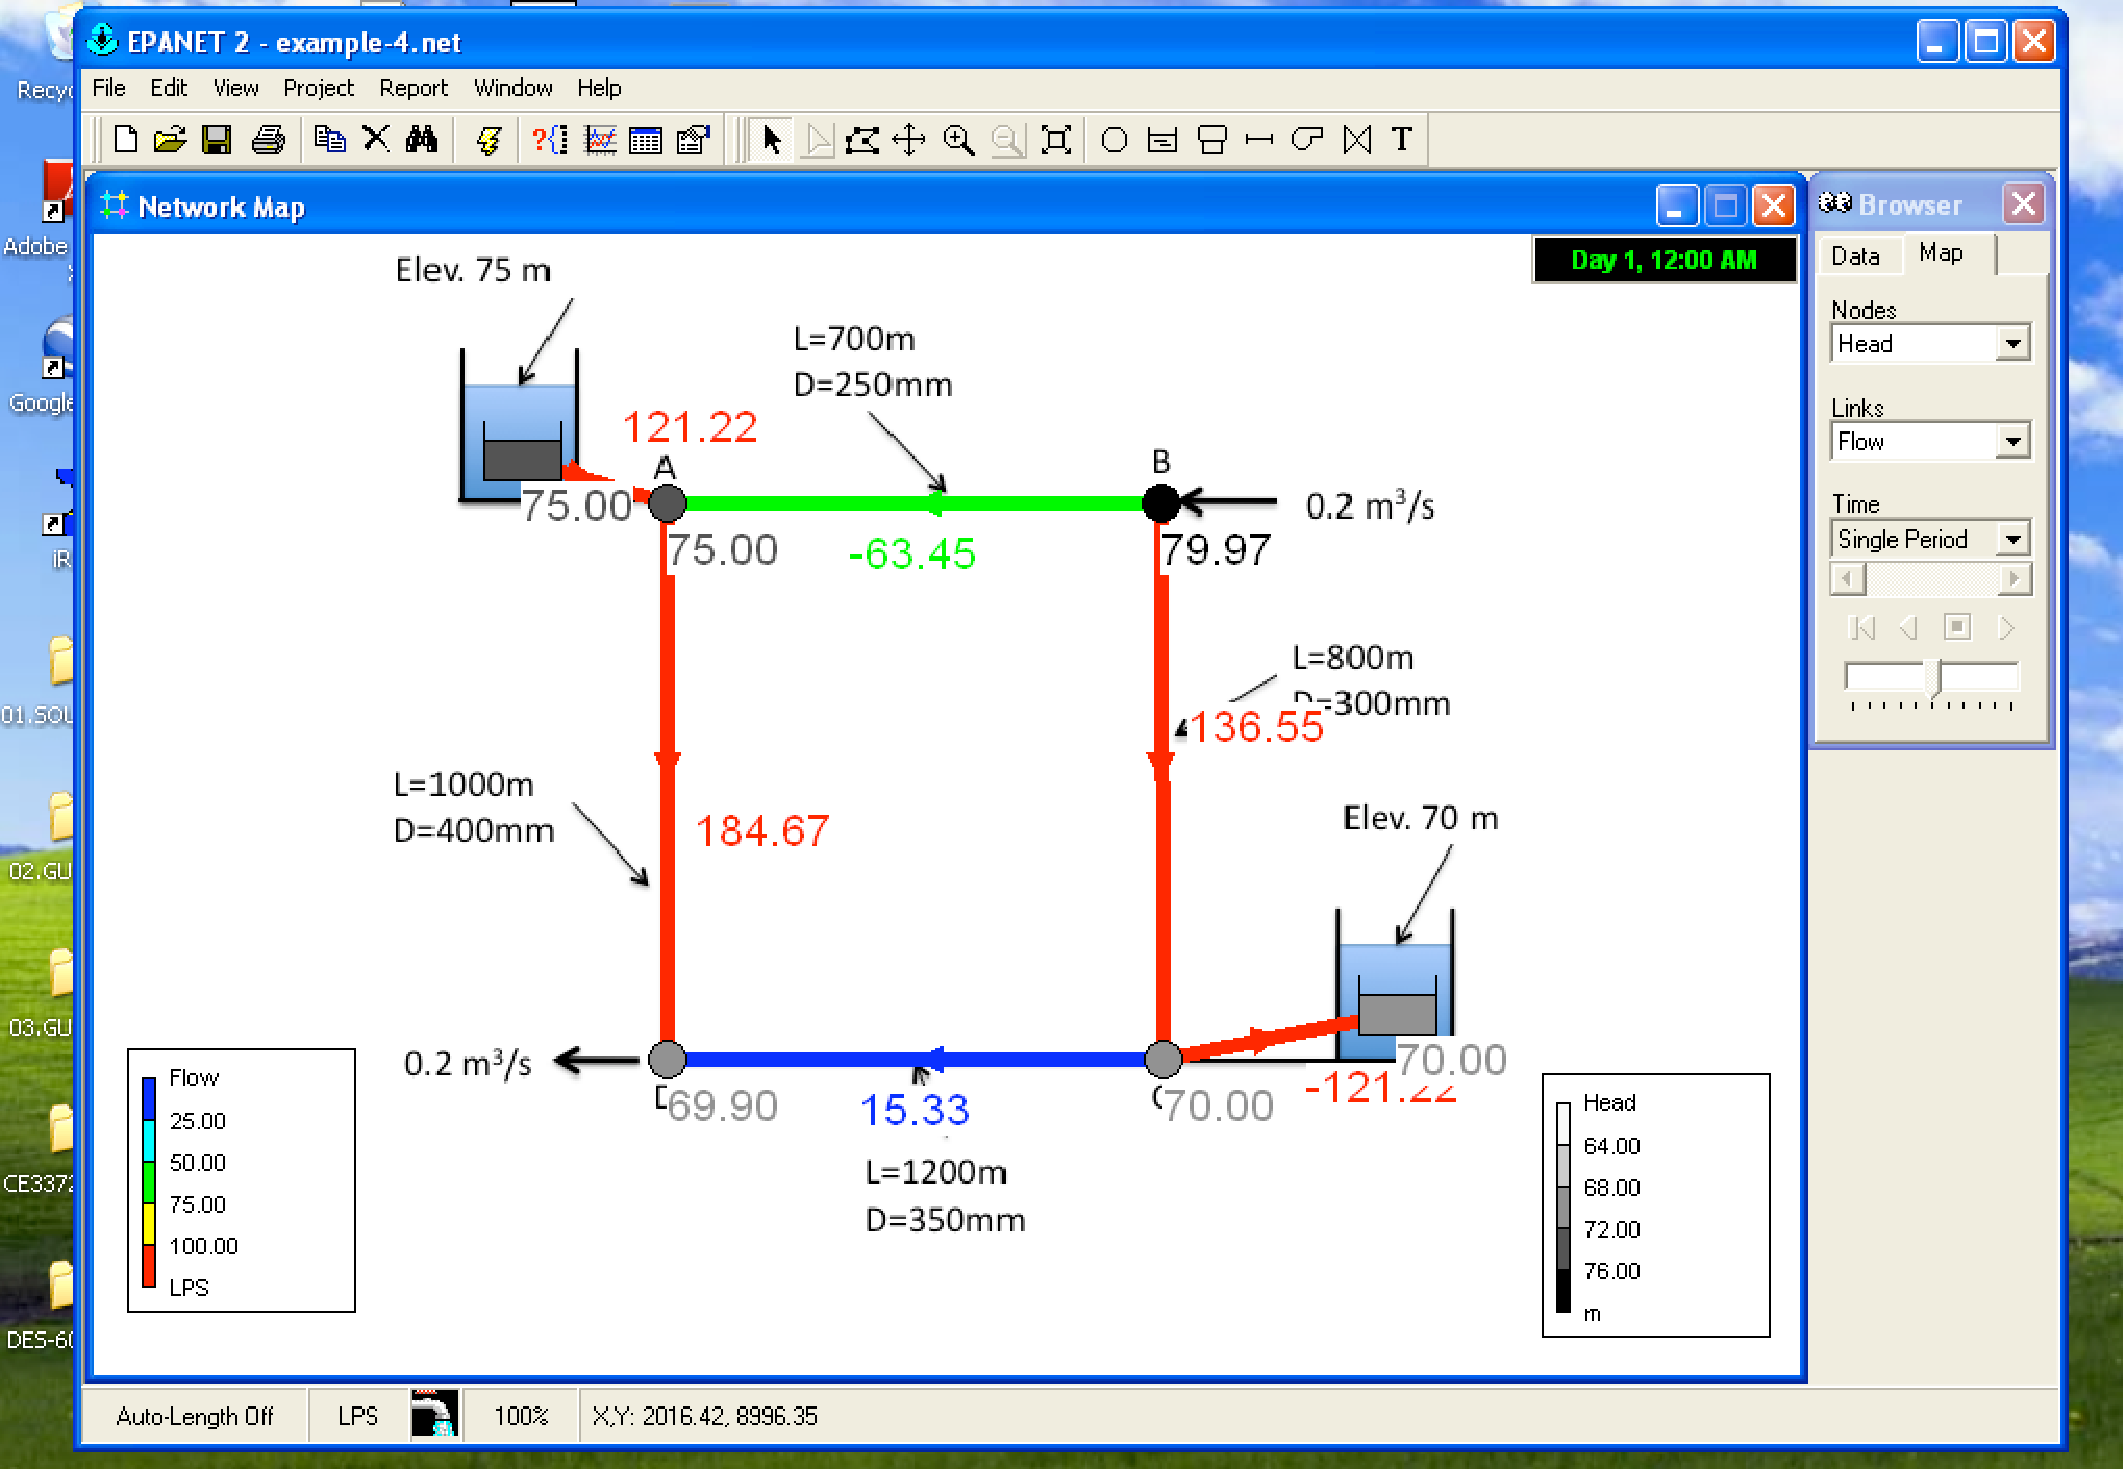
\includegraphics[width=6in]{./23-EPANETbyEXAMPLE/simple-network.pdf} 
   \caption{Solution for Example 3.  The pipes were originally straight segments, but a drawing tool in EPANET is used to follow the shape of the underlying basemap.   The training video shows the pipes as the straight lines.  The flowrates are in liters-per-second, divide by 1000 to obtain cubic-meters-per-second.}
   \label{fig:simple-network}
\end{figure}



\subsection{EPANET Modeling by Example:  Example 5}
The next example illustrates how to model a pump in EPANET.  A pump is a special ``link'' in EPANET.  This link causes a negative head loss (adds head) according to a pump curve.  In additon to a pump curve there are three other ways to model added head --- these are discussed in th eunser manual and are left for the reader to explore on their own.
\subsubsection{Example 5: Pumping Water Uphill}
Figure \ref{fig:P2-39.pdf} is a conceptual model of a pump lifting water through a 100 mm diameter, 100 meter long, ductile iron pipe from a lower to an upper reservoir.  The suction side of the pump is a 100 mm diameter, 4-meter long ductile iron pipe.  The difference in reservoir free-surface elevations is 10 meters.  The pump performance curve is given as
\begin{equation}
h_p = 15 - 0.1 Q^2
\end{equation}
where the added head is in meters and the flow rate is in liters per second (Lps).  The analysis goal is to estimate the flow rate in the system.
\begin{figure}[htbp] %  figure placement: here, top, bottom, or page
   \centering
   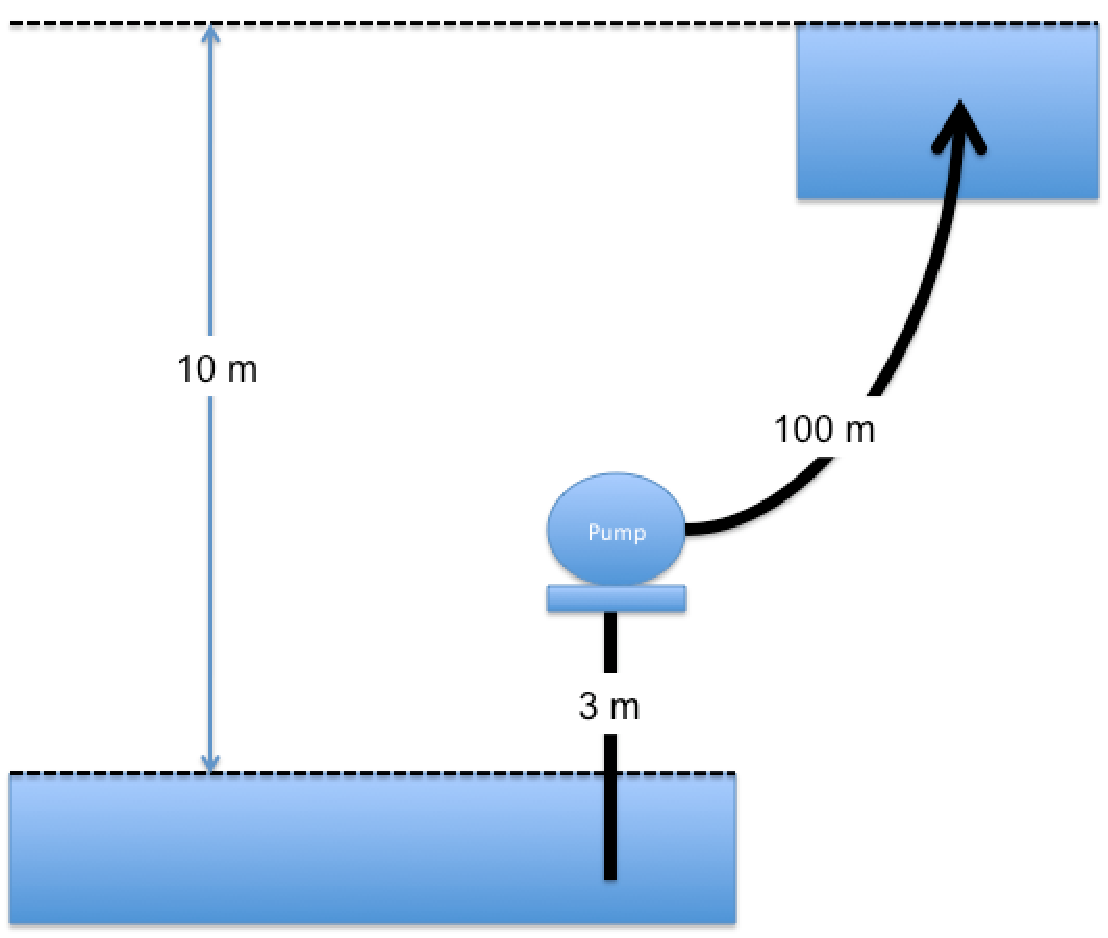
\includegraphics[width=4in]{./23-EPANETbyEXAMPLE/P2-39.pdf} 
   \caption{Example 5 conceptual model.  The pipes are 100 mm ductile iron.}
   \label{fig:P2-39.pdf}
\end{figure}

To model this situation, the engineer follows the modeling protocol already outlined, only adding the special link.
\begin{enumerate}
\item Convert the image into a bitmap, place the bitmap into a directory where the model input file will be stored.
\item Start EPANET
\item Set defaults (hydraulics = D-W,  units = LPS)
\item Import the background.
\item Select the reservoir tool.  Put two reservoirs on the map.
\item Select the node tool, put 2 nodes on the map, these represent the suction and discharge side of the pump.
\item Select the link (pipe) tool, connect the reservoirs to their nearest nodes.  
\item Select the pump tool.
\item Connect the nodes to each other using the pump link.
\item Set the total head each reservoir.
\item Set the pipe length, roughness height, and diameter in each pipe.
\item On the Data menu, select Curves.  Here is where we create the pump curve.   This problem gives the curve as an equation, we will need three points to define the curve.   Shutoff ($Q=0$), and simple to compute points make the most sense.
\item Save the input file.
\item Run the program.   
\end{enumerate}

\begin{figure}[htbp] %  figure placement: here, top, bottom, or page
   \centering
   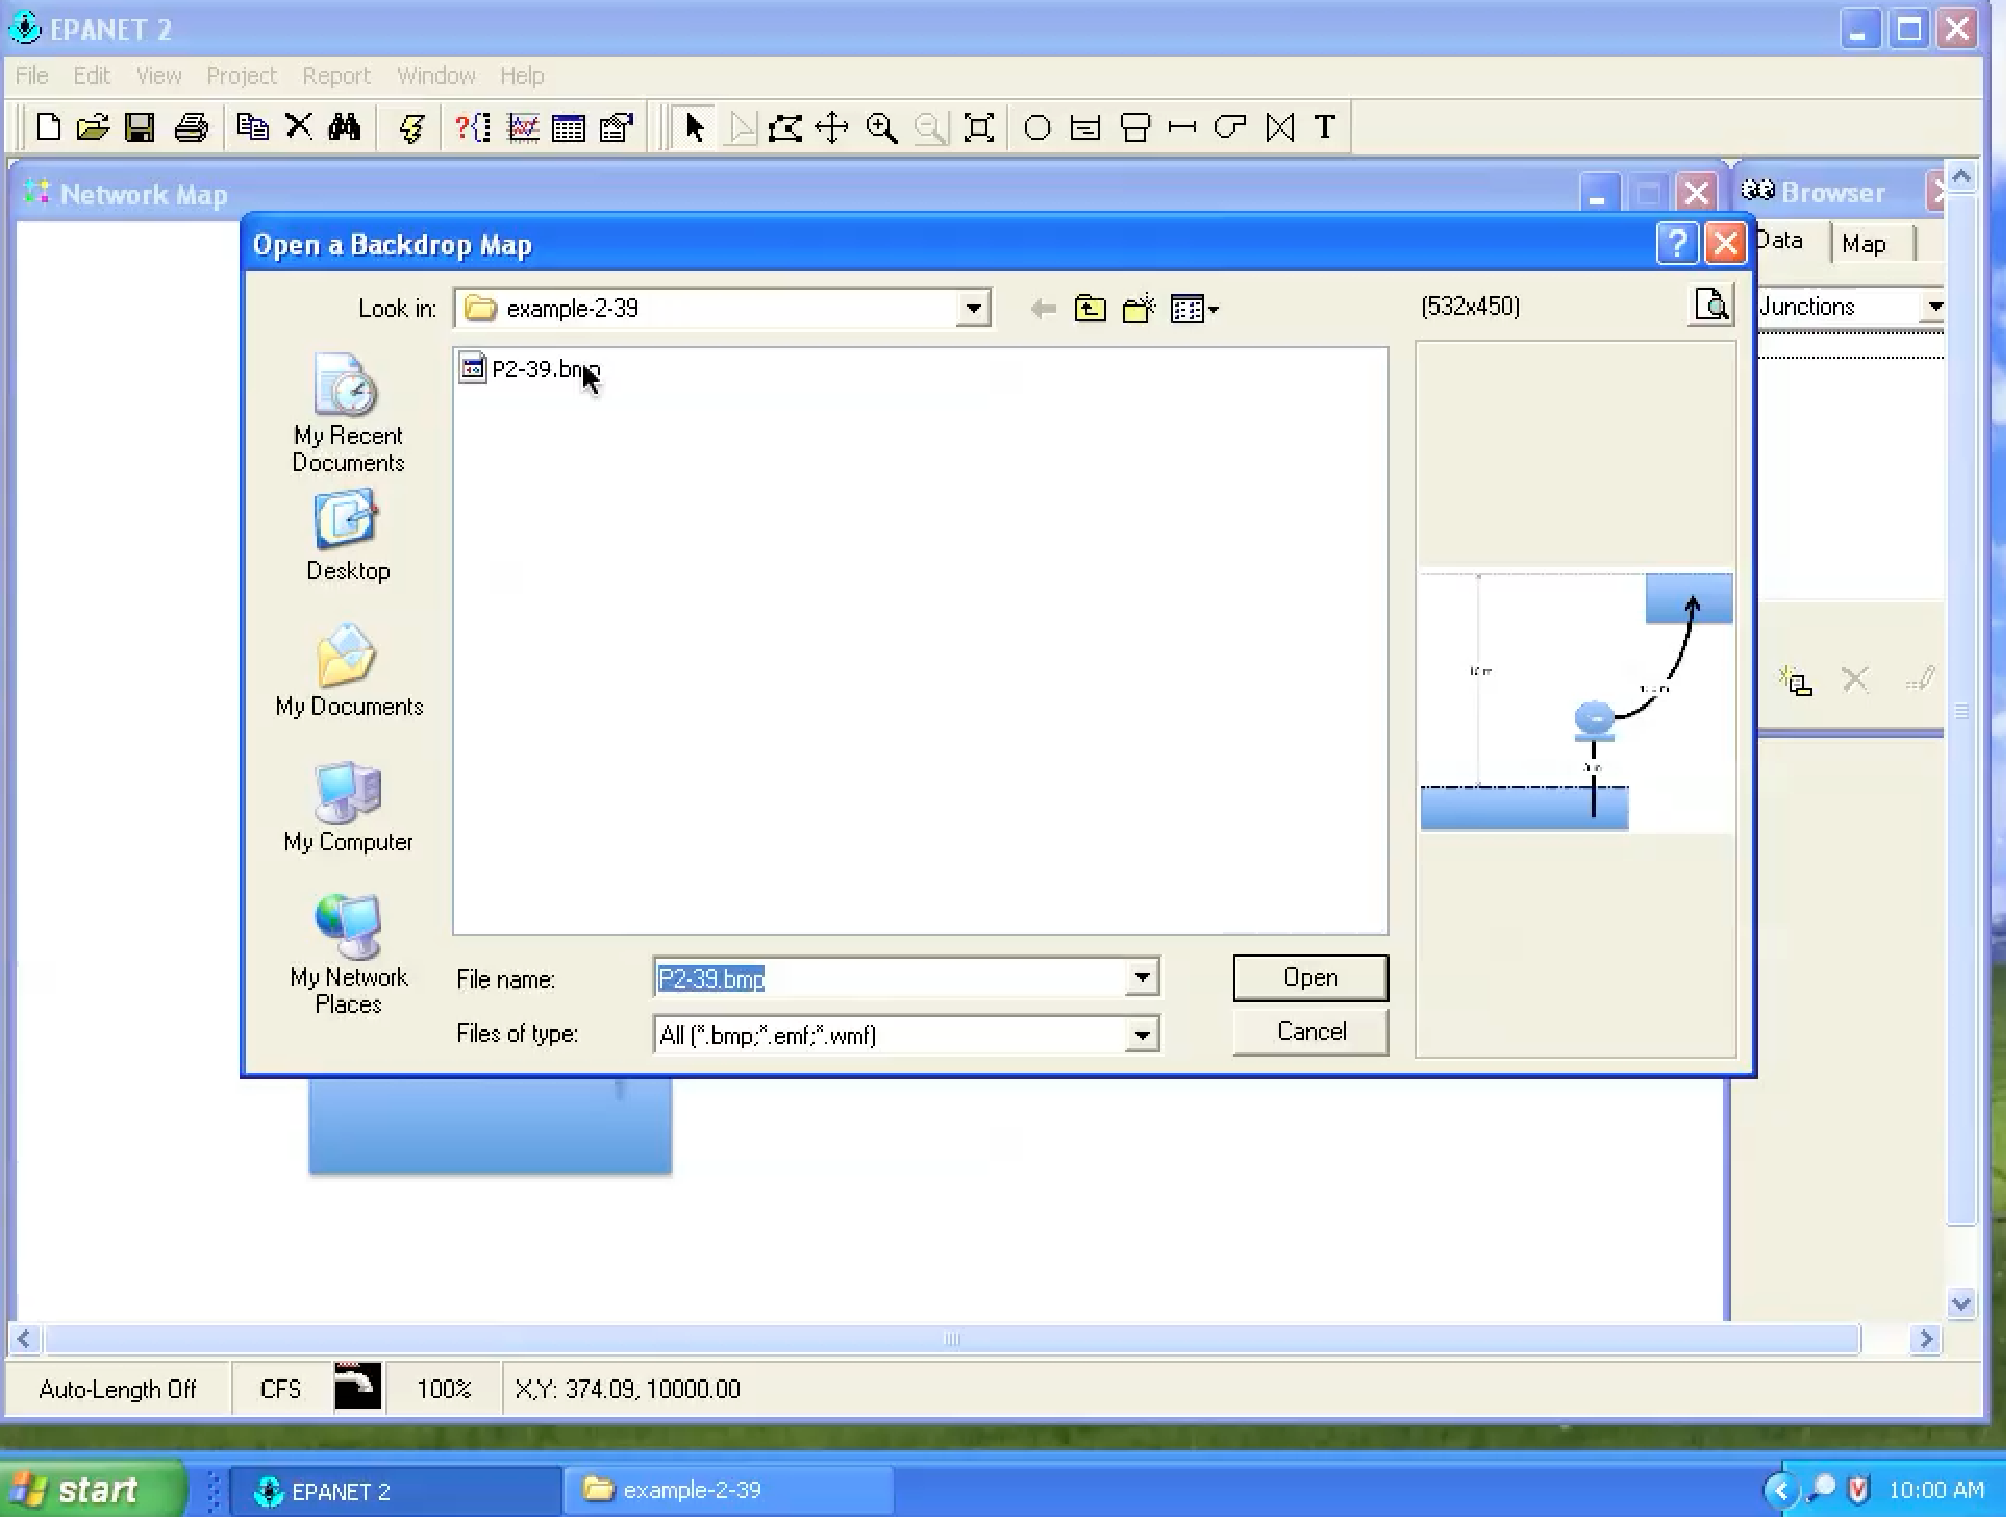
\includegraphics[width=5in]{./23-EPANETbyEXAMPLE/pump-background.pdf} 
   \caption{Example 5 select the background drawing (BMP file)}
   \label{fig:pump-background.pdf}
\end{figure}
Figure \ref{fig:pump-background.pdf} is a screen capture of loading the background image.   After the image is loaded, we can then build the hydraulic model.  The next step is to place the reservoirs.
\clearpage

\begin{figure}[htbp] %  figure placement: here, top, bottom, or page
   \centering
   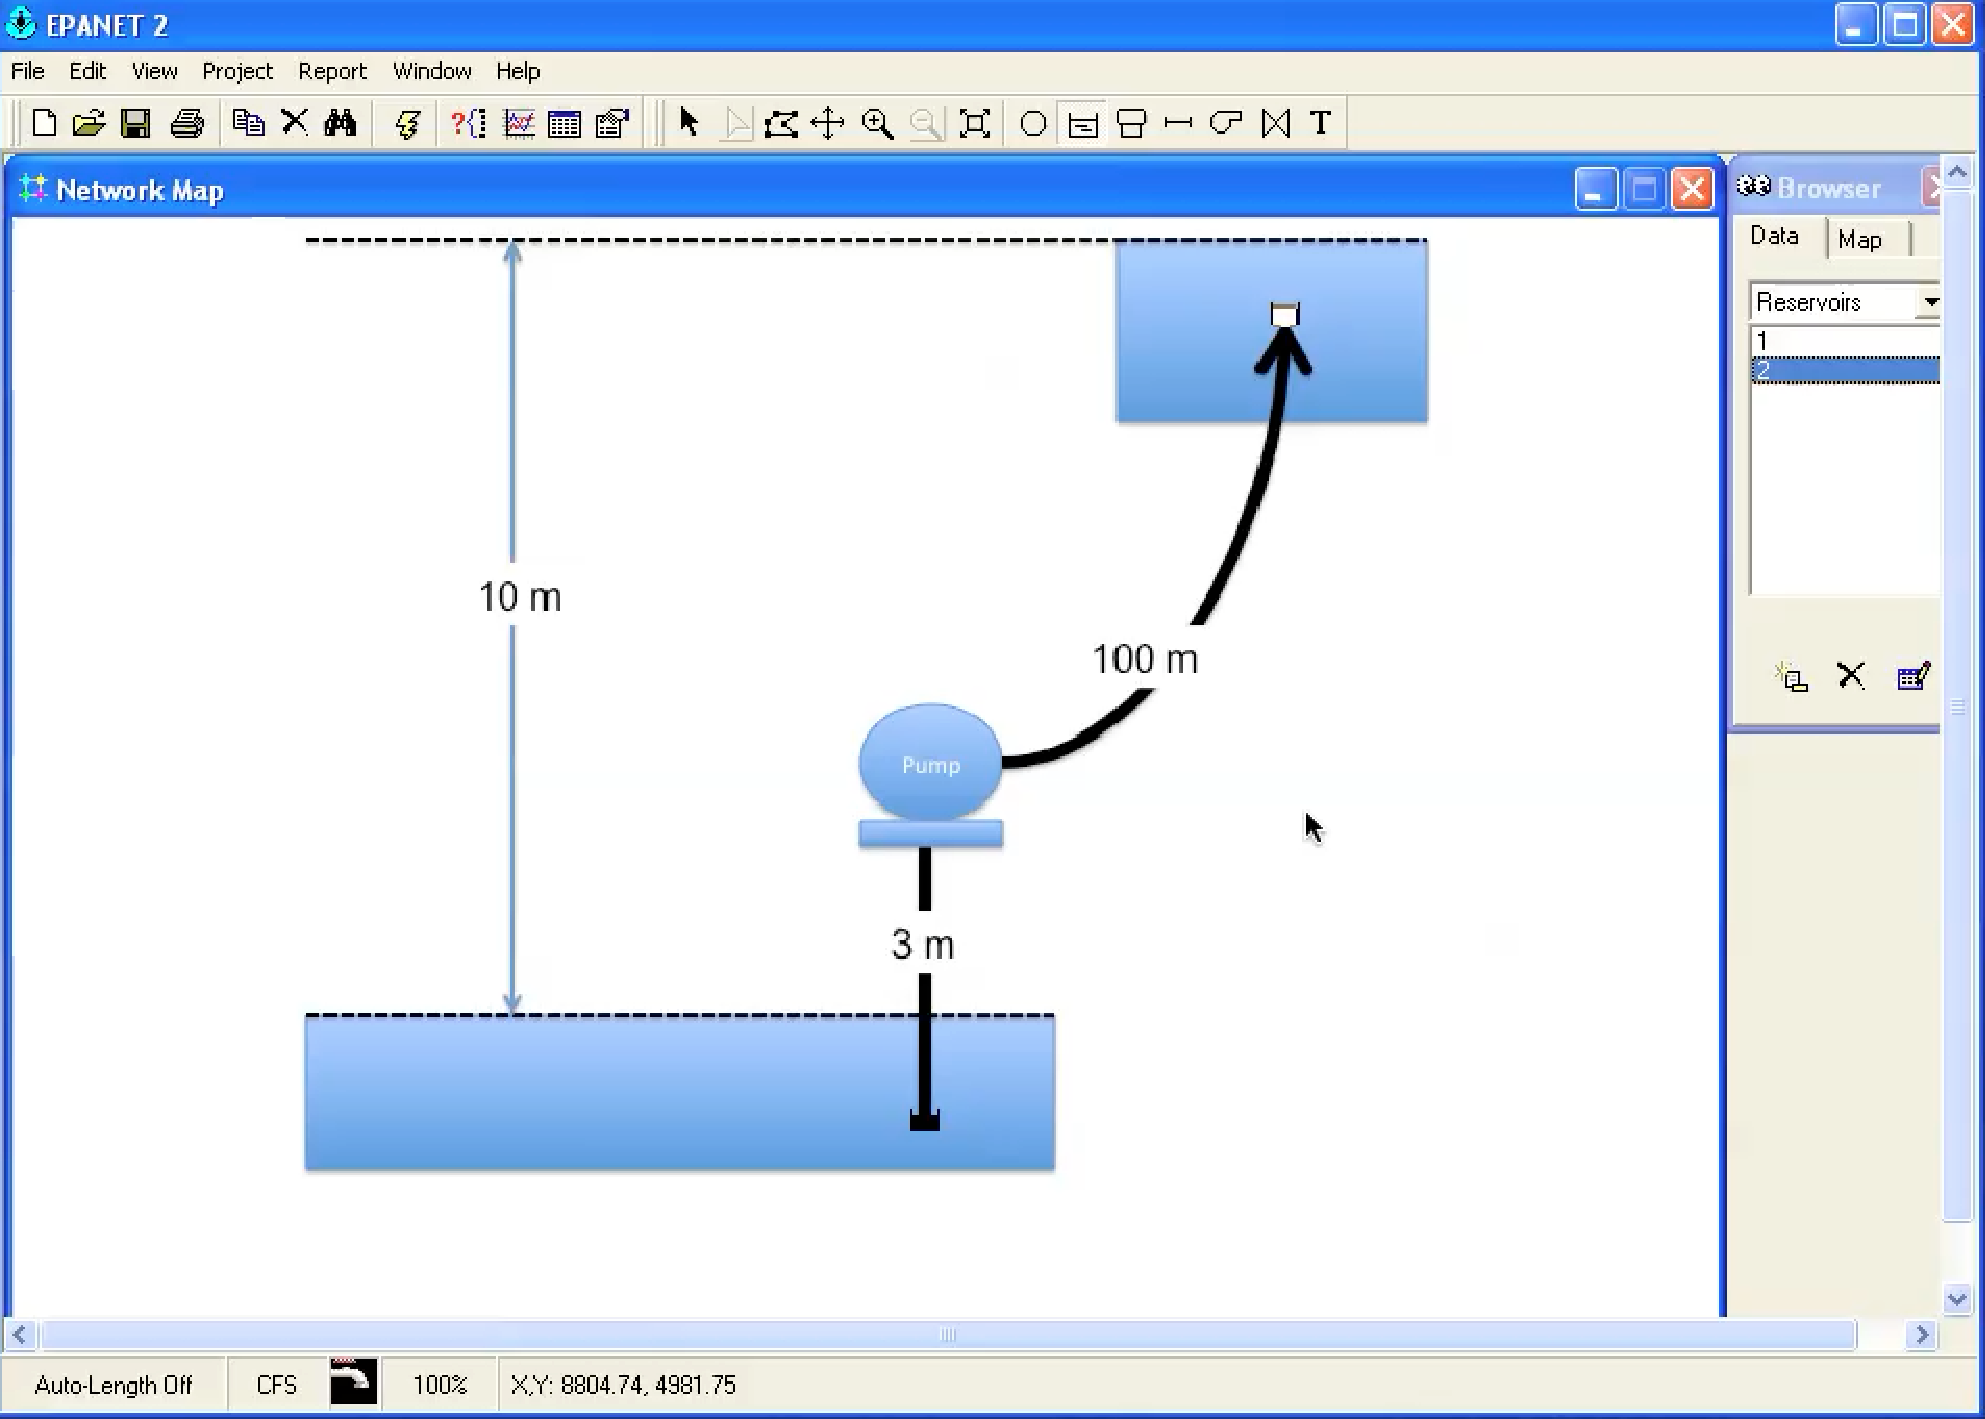
\includegraphics[width=5in]{./23-EPANETbyEXAMPLE/pump-reservoirs.pdf} 
   \caption{Example 5 place the lower and upper reservoir}
   \label{fig:pump-reservoirs.pdf}
\end{figure}
Figure \ref{fig:pump-reservoirs.pdf} is a screen capture of the reservoirs after they have been placed.  The upper reservoir will be assigned a total head 10 meters larger than the lower reservoir --- a reasonable conceptual model is to use the lower reservoir as the datum.
\newpage

\begin{figure}[htbp] %  figure placement: here, top, bottom, or page
   \centering
   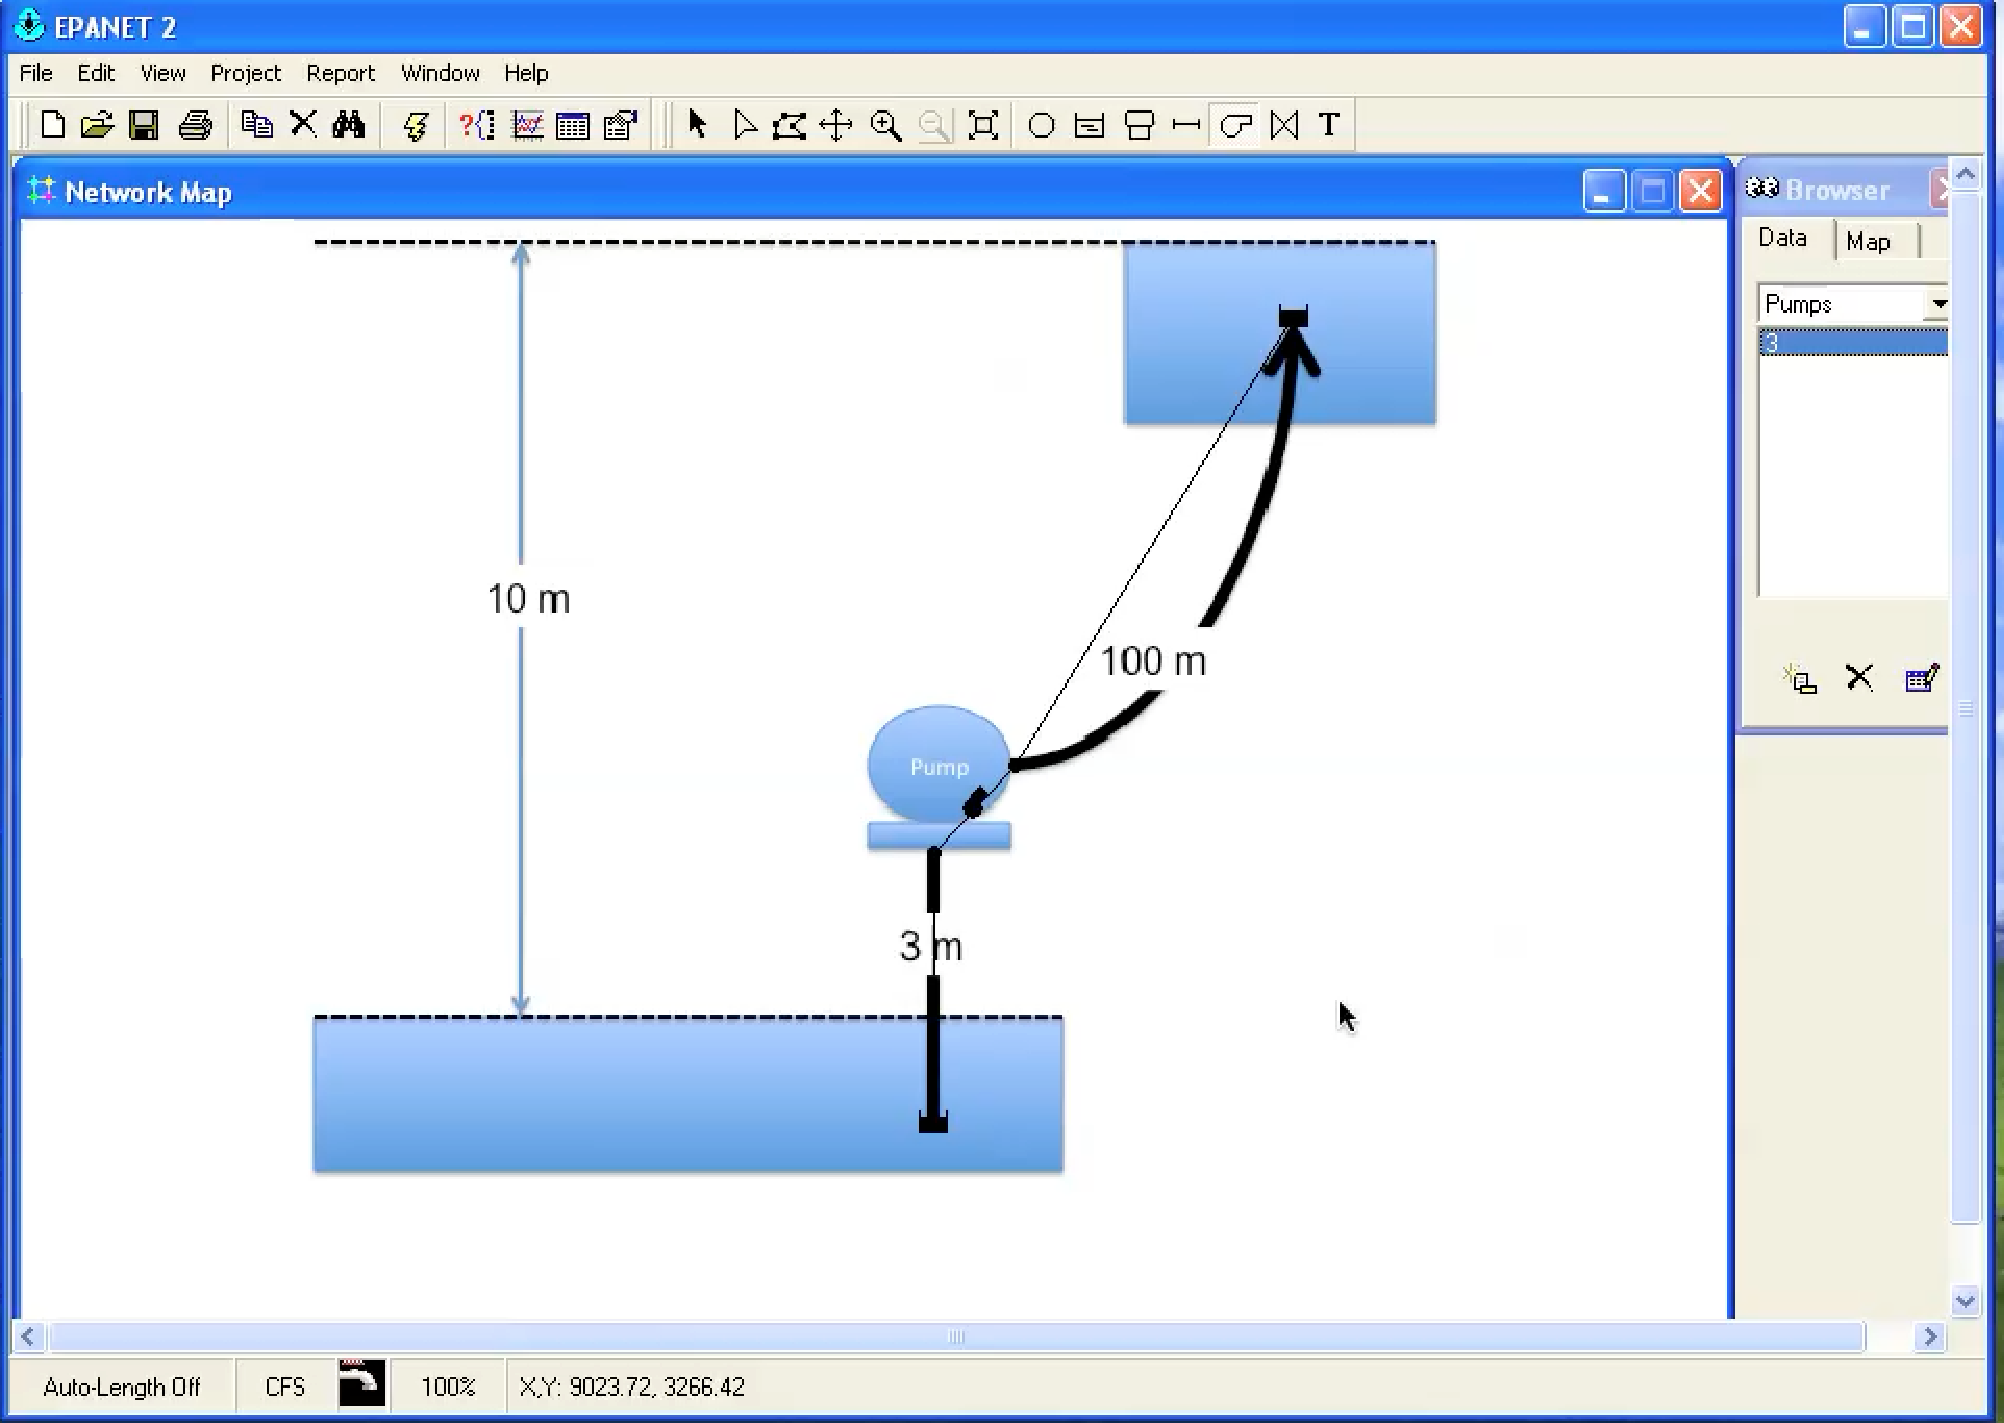
\includegraphics[width=5in]{./23-EPANETbyEXAMPLE/pump-pump.pdf} 
   \caption{Example 5 place the nodes, pipes, and the pump link.}
   \label{fig:pump-pump.pdf}
\end{figure}
Figure \ref{fig:pump-pump.pdf} is a screen capture of model just after the pump is added.   The next steps are to set the pipe lengths (not shown) and the reservoir elevations (not shown).   Finally, the engineer must specify the pump curve.
\newpage

\begin{figure}[htbp] %  figure placement: here, top, bottom, or page
   \centering
   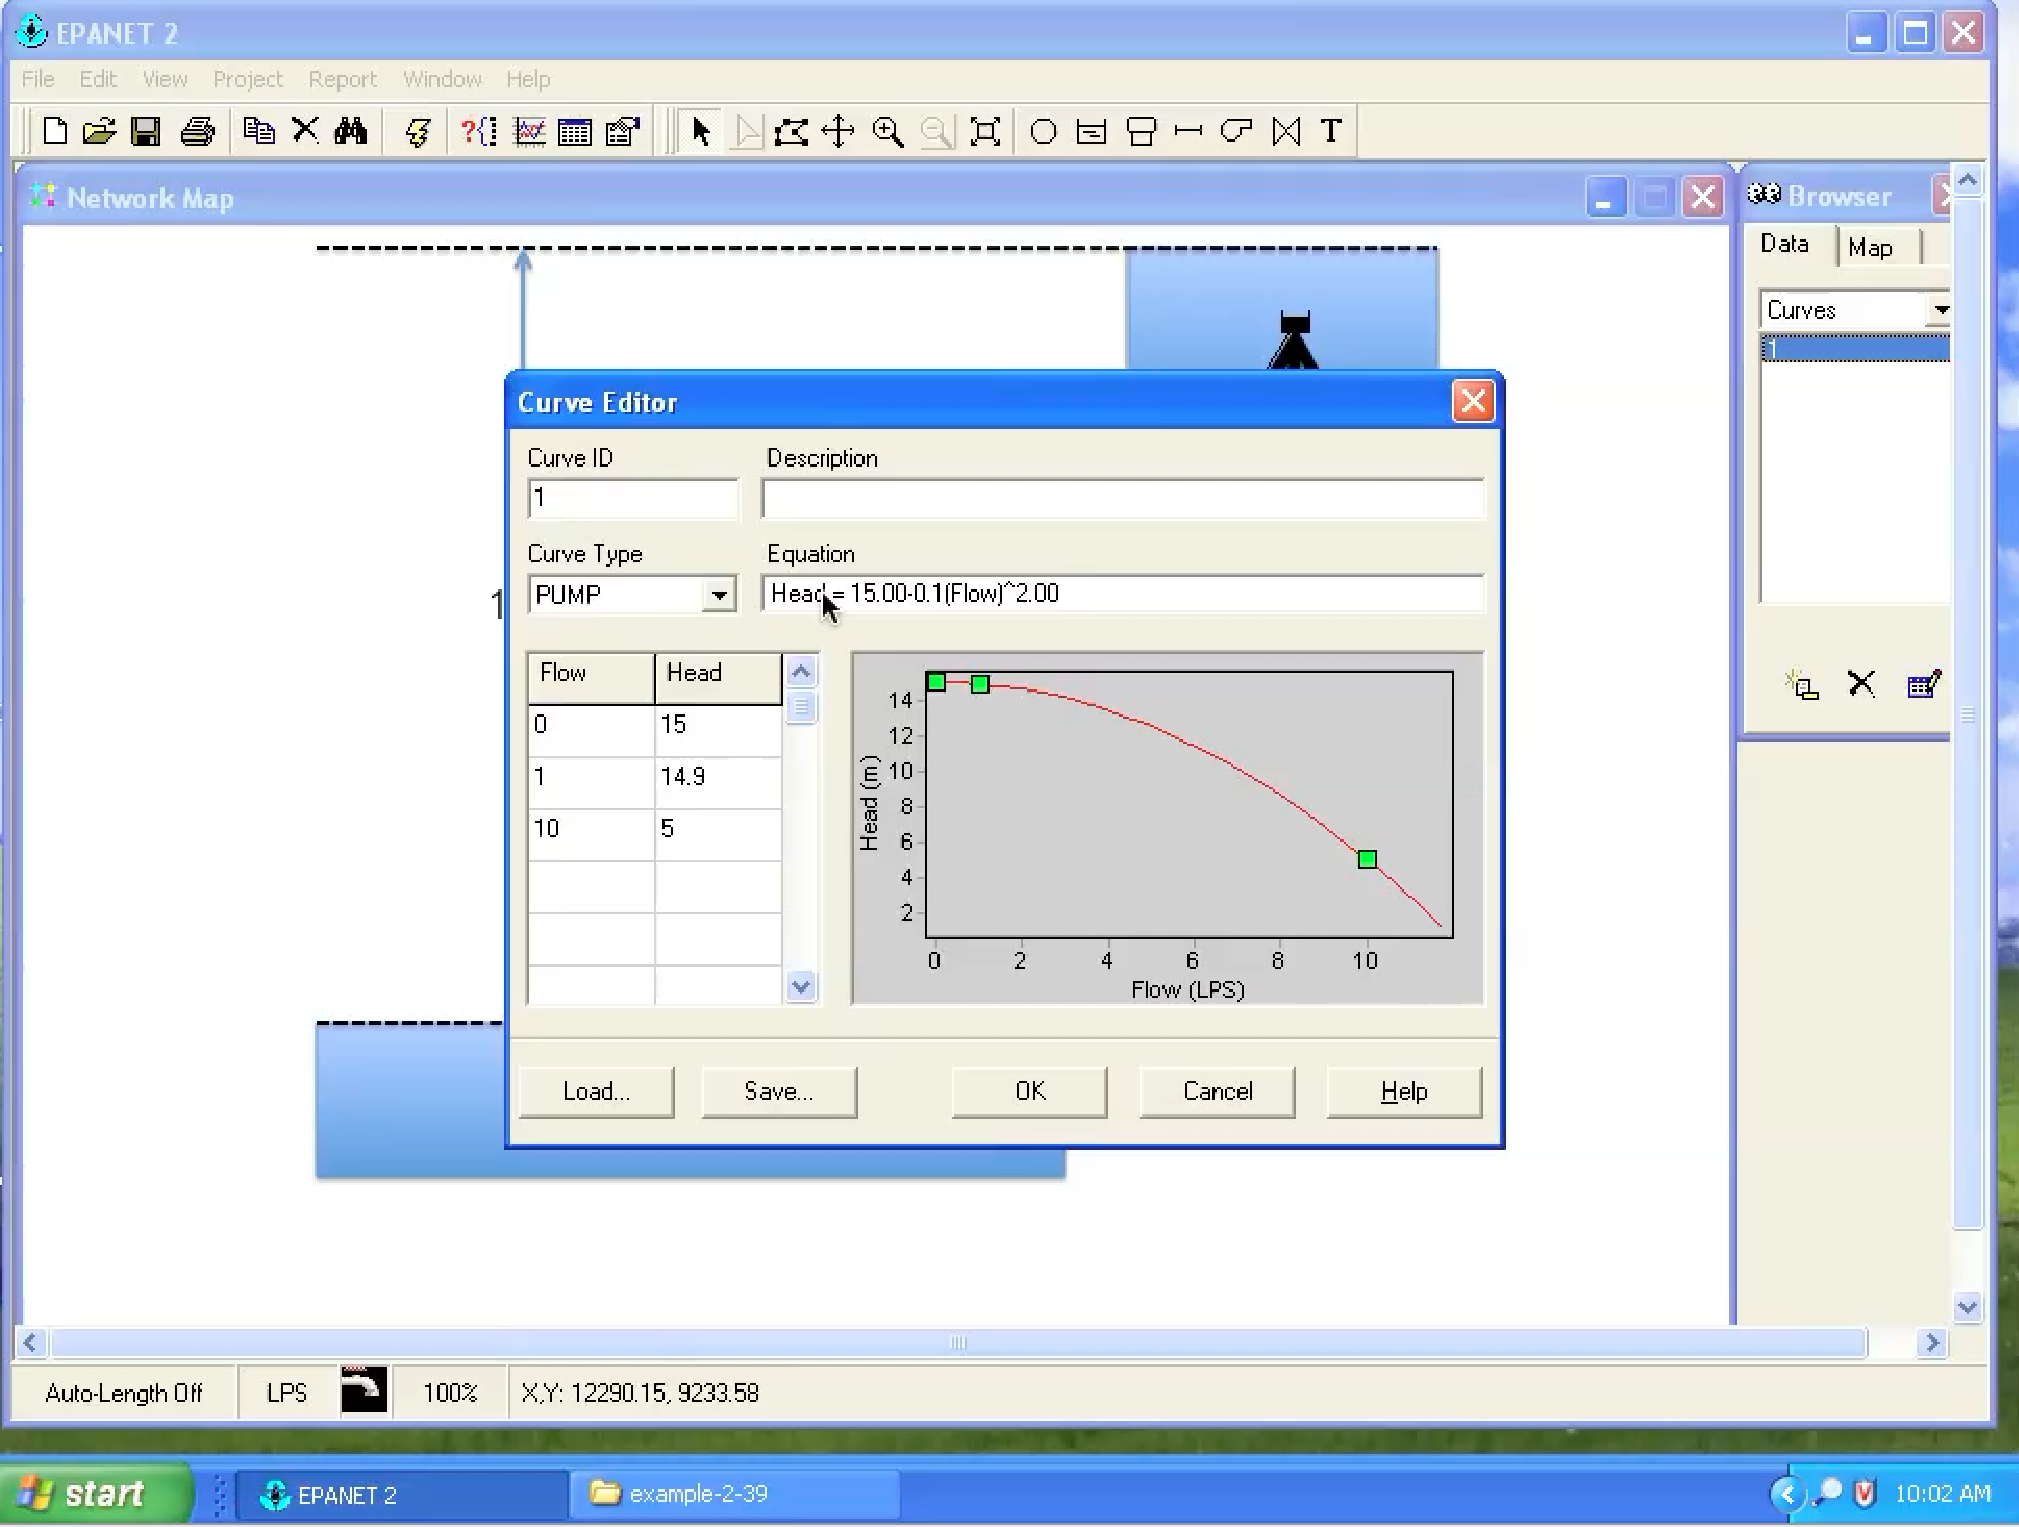
\includegraphics[width=5in]{./23-EPANETbyEXAMPLE/pump-curve.pdf} 
   \caption{Example 5 pump curve entry dialog box.  Three points are entered and the curve equation is created by the program.}
   \label{fig:pump-curve.pdf}
\end{figure}
Figure \ref{fig:pump-curve.pdf} is a screen capture of the pump curve data entry dialog box.   Three points on the curve were selected and entered into the tabular entry area on the left of the dialog box, then the curve is created by the program.  The equation created by the program is the same as that of the problem -- hence we have the anticipated pump curve.
\newpage

Next the engineer associates the pump curve with the pump as shown in Figure \ref{fig:set-curve}.
\begin{figure}[htbp] %  figure placement: here, top, bottom, or page
   \centering
   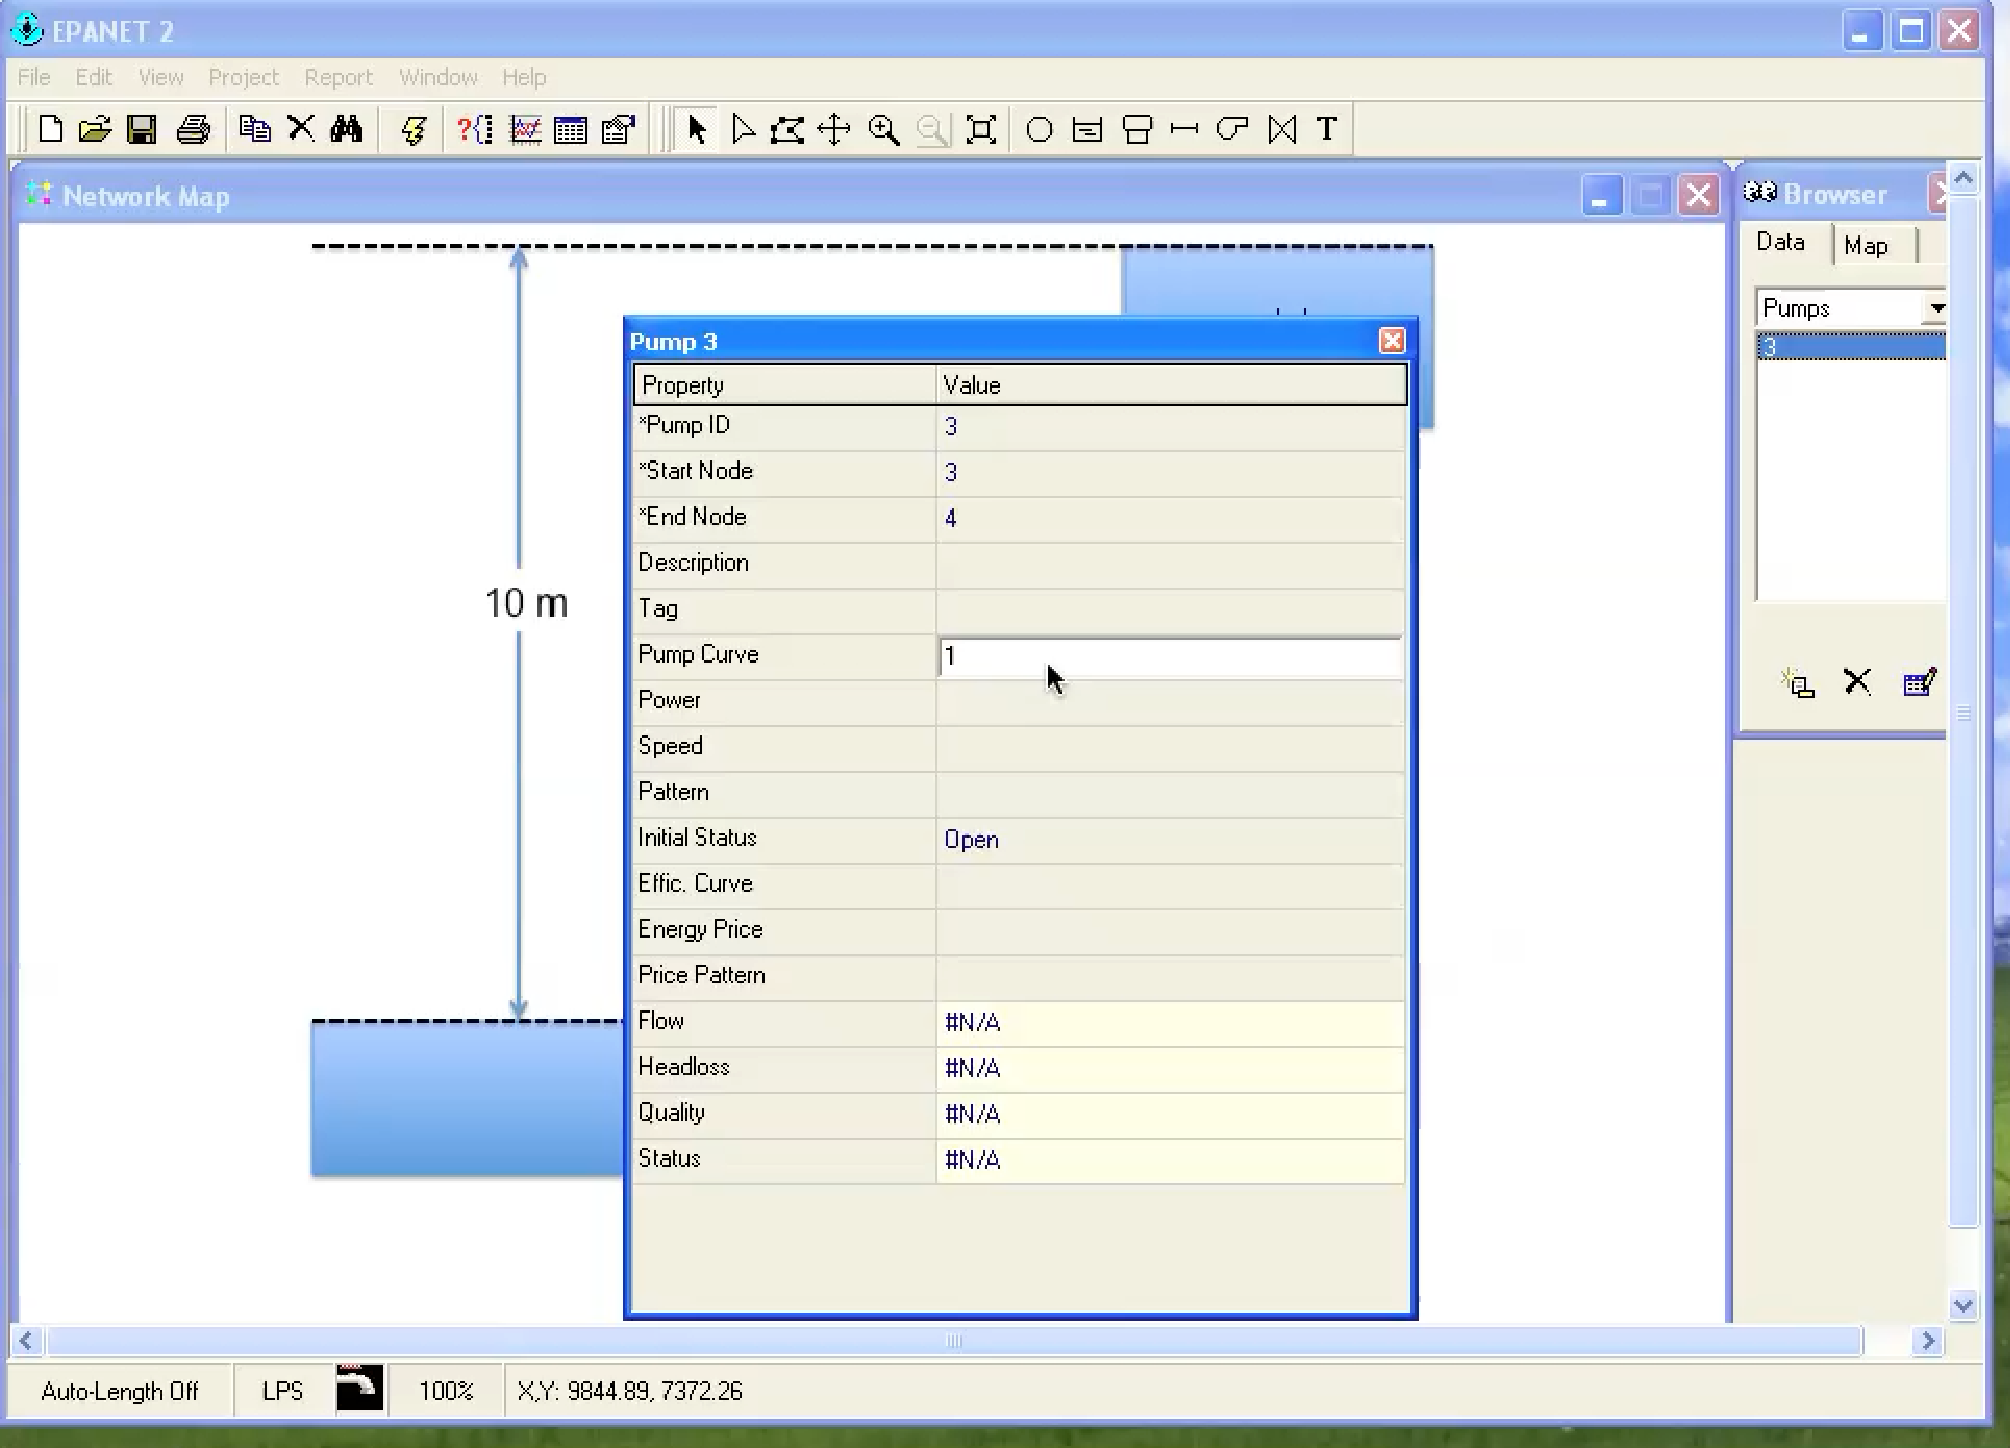
\includegraphics[width=5in]{./23-EPANETbyEXAMPLE/set-curve.pdf} 
   \caption{Setting the pump curve.}
   \label{fig:set-curve}
\end{figure}

Upon completion of this step, the program is run to estimate the flow rate in the system.
\clearpage

\subsection{EPANET Modeling by Example:  Example 6}
Example 6 is an extended period simulation -- the files will simply be provided; the concept is well described in most hydraulics textbooks, as well as in the EPANET Documentation, however in the interest of time, it is left to the reader to download and run an extended period simulation model.  The goal (for the seminar) is to have a working model of some complexity to explore the other tools discussed later.
\clearpage
%%%%%%%%%%%%%%%%%%%%%%%%%%%%%%%%%%%%%%%%%%%%%%%%%%
%%%%%%%%%%%%%%%%%%%%%%%%%%%%%%%%%%%%%%%%%%%%%%%%%%
%%%%%%%%%%%%%%%%%%%%%%%%%%%%%%%%%%%%%%%%%%%%%%%%%%

\subsection{The Respec Interface}
The \url{url to install video} shows how to download and install EPANET onto your computer using the newer Respec GUI.  This interface was built to be GIS aware and facilitate integration of an asset management database and the simulation software.  

\subsubsection{Installing the NewUI}
The pre-release of the NewUI is located on a GitHub repository at
\url{https://github.com/USEPA/SWMM-EPANET_User_Interface/releases}.

Figure \ref{fig:GitHubRepoPage} is a screen capture of the page.
   
\begin{figure}[htbp] %  figure placement: here, top, bottom, or page
   \centering
   \includegraphics[width=4.5in]{./23-EPANETbyEXAMPLE/Lesson6/chapter6figures/GitHubRepoPage.jpg} 
   \caption{Git Hub Repository Page for the NewUI.}
   \label{fig:GitHubRepoPage}
\end{figure}

The file named \texttt{EPANET-UI-MTP4r1.exe} is a PC installer file that can be downloaded and installed.   
Select the file and begin the download.

On the computer that is used for the screen captures in this document the following were installed in advance of the NewUI.
\begin{enumerate}
\item Python 3 (I used the Anaconda installer and installed the 64-bit Python).
\item QGIS.  I used both the stand-alone \texttt{QGIS-OSGeo4W-2.18.8-1-Setup-x86\_64.exe} and the over-the-wire \texttt{osgeo4w-setup-x86\_64.exe} installer.
\end{enumerate}

Python probably needs to be present, because the NewUI uses python scripts to access certain QGIS \texttt{.DLL} files for the interface.
QGIS is handy because an environment variable needs to be set to point to a directory that contains a collection of \texttt{.CSV} files -- these are located in the QGIS program.

The next series of screen captures document the installation from just after the download, to setting the environment variable.

Figure \ref{fig:win10InstallScreen} is the install screen on Windows 10 where the OS is requesting permission to write to the disk.  The user would choose yes.

\begin{figure}[htbp] %  figure placement: here, top, bottom, or page
   \centering
   \includegraphics[width=4.5in]{./23-EPANETbyEXAMPLE/Lesson6/chapter6figures/win10InstallScreen.jpg} 
   \caption{Windows 10 Installer Security Panel -- Choose Yes}
   \label{fig:win10InstallScreen}
\end{figure}
\clearpage

Figure \ref{fig:win10Install2} is the first of several installer dialog boxes.  The user would select next to begin the installation.

\begin{figure}[h!] %  figure placement: here, top, bottom, or page
   \centering
   \includegraphics[width=4.5in]{./23-EPANETbyEXAMPLE/Lesson6/chapter6figures/win10Install2.jpg} 
   \caption{Installer Dialog Box}
   \label{fig:win10Install2}
\end{figure}

Figure \ref{fig:win10Install3} is the next of several more installer dialog boxes.  The user would select next to accept the install defaults and continue through a series of such screens.

\begin{figure}[h!] %  figure placement: here, top, bottom, or page
   \centering
   \includegraphics[width=4.5in]{./23-EPANETbyEXAMPLE/Lesson6/chapter6figures/win10Install3.jpg} 
   \caption{Installer Dialog Box -- Accept the Defaults}
   \label{fig:win10Install3}
\end{figure}

\clearpage
%\begin{figure}[htbp] %  figure placement: here, top, bottom, or page
%   \centering
%   \includegraphics[width=4in]{./23-EPANETbyEXAMPLE/Lesson6/chapter6figures/win10Install4.jpg} 
%   \caption{Installer Dialog Box -- Accept the Defaults}
%   \label{fig:win10Install4}
%\end{figure}

\begin{figure}[h!] %  figure placement: here, top, bottom, or page
   \centering
   \includegraphics[width=5in]{./23-EPANETbyEXAMPLE/Lesson6/chapter6figures/win10Install5.jpg} 
   \caption{Installer Dialog Box -- Ready for the Install}
   \label{fig:win10Install5}
\end{figure}

Figure \ref{fig:win10Install5} is the installer ready to begin the install.  In the figure, we have selected a default installation and the creation of a desktop alias.  The user would select install and the installation would begin.   The program installs pretty fast, less than a minute.

\begin{figure}[h!] %  figure placement: here, top, bottom, or page
   \centering
   \includegraphics[width=5in]{./23-EPANETbyEXAMPLE/Lesson6/chapter6figures/win10Install6.jpg} 
   \caption{Installed -- Ready to Start}
   \label{fig:win10Install6}
\end{figure}
Figure \ref{fig:win10Install6} is the completion screen, ready to start the program.
\clearpage
\begin{figure}[h!] %  figure placement: here, top, bottom, or page
   \centering
   \includegraphics[width=6in]{./23-EPANETbyEXAMPLE/Lesson6/chapter6figures/win10Install7.jpg} 
   \caption{Initial run -- interface loads, but notice the error message in the script.  I was able to use the interface, but dealing with the error now is best.  We will have to set an environment variable.}
   \label{fig:win10Install7}
\end{figure}

Figure \ref{fig:win10Install7} is the initial run of the NewUI.  While it seems OK, notice the error message regarding \texttt{GDAL\_DAT} directories.  In my case, because GIS is a novelty to me, I don't have an existing environment for the \texttt{GDAL} libraries.  The next several figures go through how to set the variable on my machine, the steps would be similar on user machines, with the variable pointing to the correct location.  There might be some issue if the user cannot set variables in a network environment and they would need the system administrator to set the variable.
The variable can also be set in a script.

In Windows 10, the user would right-click in the lower left hand corner of their desktop, on top of the window pane.
A menu column should appear, and the user will select SYSTEM.
Figure \ref{fig:win10Install8} is a screen capture showing these steps.

Upon entry into the system setting dialog box there is a link called ADVANCED SYSTEM SETTINGS in the left column. 
On my machine, it is the bottom item.
Select ADVANCED SYSTEM SETTINGS
The selection opens another dialog box called SYSTEM PROPERTIES.  
The bottom selection button is labeled ENVIRONMENT VARIABLES.
Select this button to get to the next dialog box which will allow us to set the requisite variable.

\begin{figure}[h!] %  figure placement: here, top, bottom, or page
   \centering
   \includegraphics[width=5in]{./23-EPANETbyEXAMPLE/Lesson6/chapter6figures/win10Install8.jpg} 
   \caption{Access the environment variable dialog.   Right-click in the lower left hand corner.  Then select system.}
   \label{fig:win10Install8}
\end{figure}

\newpage Figure \ref{fig:win10Install9} is a screen capture of these steps.   
\begin{figure}[h!] %  figure placement: here, top, bottom, or page
   \centering
   \includegraphics[width=5in]{./23-EPANETbyEXAMPLE/Lesson6/chapter6figures/win10Install9.jpg} 
   \caption{In System, select ``Advanced System Settings.''   Then in the settings dialog, select ``Environment Variables.''}
   \label{fig:win10Install9}
\end{figure}

\clearpage
Once the user has the ENVIRONMENT VARIABLE dialog box open, then we can set the variable.
In the lower panel are the SYSTEM VARIABLES, and the user will select NEW SYSTEM VARIABLE.
The new variable dialog box opens and we type the variable name, in this case \texttt{GDAL\_DAT}.
Next we need to set its value.
The value is a path to the directory where the particular data structures reside.  
On my machine the variable is set to \texttt{C:/OSGeo4W64/share/epsg\_csv}.

Other users will probably have different paths. 
Figure \ref{fig:win10Install10} is a screen capture illustrating these steps.

\begin{figure}[h!] %  figure placement: here, top, bottom, or page
   \centering
   \includegraphics[width=6in]{./23-EPANETbyEXAMPLE/Lesson6/chapter6figures/win10Install10.jpg} 
   \caption{In Environment Variables, select ``NEW SYSTEM VARIABLE.''  As an aside, I tried to set the variable as a user environment variable (the upper part of the dialog) and did not shake the error.  So the program is expecting a system variable that points to the directory \texttt{epsg\_csv}.   The directory is part of the Geospatial Data Abstraction Library and may be located in different palces on other machines.  In particular, if a user already has ArcGIS, then conceivably the interface could access that directory.}
   \label{fig:win10Install10}
\end{figure}

After the selection the dialog box reports the variable and its value (before we select OK and get out of the system menu).
Figure \ref{fig:win10Install11} illustrates the result.  
From this condition, the user should select OK and exit in reverse the various system dialog boxes until they are back to their desktop with the NewUI still running.

\begin{figure}[h!] %  figure placement: here, top, bottom, or page
   \centering
   \includegraphics[width=4in]{./23-EPANETbyEXAMPLE/Lesson6/chapter6figures/win10Install11.jpg} 
   \caption{After selecting the directory, the environment variable points to the directory.  Now ready to close the settings dialogs and return to the interface.}
   \label{fig:win10Install11}
\end{figure}

The next step is to exit the NewUI and restart the program.  Upon the restart the error should be addressed and we are ready to build models.\footnote{The program runs OK with the error in place, but seemed to work better when the error was addressed.}

\begin{figure}[h!] %  figure placement: here, top, bottom, or page
   \centering
   \includegraphics[width=5in]{./23-EPANETbyEXAMPLE/Lesson6/chapter6figures/win10Install13.jpg} 
   \caption{Returned to the NewUI and closed the program.  Then restart, and the error is addressed.}
   \label{fig:win10Install13}
\end{figure}
\clearpage

\subsection{Verify the Install}
The easiest way to verify the install is to open one of the examples supplied with EPANET.   
They are located in some variant of \texttt{C:/ProgramFiles/EPANET-UI/Examples}.

Figure \ref{fig:enNewUIOpenFile} illustrates selecting a file from the examples directory.
On my machine I have already palced a few extra examples, the default install will only have three (3) examples.

\begin{figure}[h!] %  figure placement: here, top, bottom, or page
   \centering
   \includegraphics[width=6in]{./23-EPANETbyEXAMPLE/Lesson6/chapter6figures/enNewUIOpenFile.jpg} 
   \caption{Open an example file supplied with the program.}
   \label{fig:enNewUIOpenFile}
\end{figure}

Upon opening the interface displays the image shown below in Figure \ref{fig:en2example1}.
The example has a dozen pipes, a storage tank, supply reservoir, and a pump.
The next step to verify the installation is to try to run EPANET from the NewUI.

Like the OldUI we can either choose to click on the ``lightning bolt'' icon, or choose RUN SIMULATION.
The selection of RUN SIMULATION from the PROJECT menu tab is illustrated in Figure \ref{fig:en2example1RunSimulation}.


\clearpage
\begin{figure}[h!] %  figure placement: here, top, bottom, or page
   \centering
   \includegraphics[width=5in]{./23-EPANETbyEXAMPLE/Lesson6/chapter6figures/en2example1.jpg} 
   \caption{Example 1 file supplied with the program.}
   \label{fig:en2example1}
\end{figure}


\begin{figure}[h!] %  figure placement: here, top, bottom, or page
   \centering
   \includegraphics[width=5in]{./23-EPANETbyEXAMPLE/Lesson6/chapter6figures/en2example1RunSimulation.jpg} 
   \caption{Example 1 RUN SIMULATION.}
   \label{fig:en2example1RunSimulation}
\end{figure}
Upon completion of the simulation, we can use the interface to interrogate the resultant database, for example, Figure \ref{fig:en2example1Plot} is a plot of discharge in the pipe connecting the pump to the network.
It was constructed by activating SELECT OBJECT in the EDIT menu.
The selecting the pipe object (double click to be sure the object ID is correct -- the example does not have pipe labels activated).   
Then selecting the time series icon in the interface.
The user then selects the plot type (TIME SERIES), the object type (LINK), the object ID (Link 10), the plot parameter (FLOW), and finally OK.
\begin{figure}[h!] %  figure placement: here, top, bottom, or page
   \centering
   \includegraphics[width=5in]{./23-EPANETbyEXAMPLE/Lesson6/chapter6figures/en2example1Plot.jpg} 
   \caption{Example 1 Plot of Flow in Pipe ID=10.}
   \label{fig:en2example1Plot}
\end{figure}

The next part of this document illustrates building simple models in the interface without regards to geo-referencing.
These examples are based on the examples presented in \\ \url{http://www.rtfmps.com/university-courses/ce-3372/3-Readings/EPANETbyExample/} and are illustrative of elementary examples used in teaching the use of EPANET as a hydraulic tool to college students.

Additional pipe network specific training materials can be found in Lectures 9 through 13 located at
\url{http://www.rtfmps.com/university-courses/ce-3372/1-Lectures/}

\clearpage


%%%%%%%%%%%%%%%%%%%%%%%%%
\subsection{EPA-NET Modeling by Example}
EPA-NET models are comprised of nodes, links,and reservoirs.    
Pumps are treated as special links (that add head).  
Valves are also treated as special links depending on the valve types.  
All models must have a reservoir (or storage tank).

\subsubsection{Defaults}
The program has certain defaults that should be set at the beginning of a simulation.  
The main defaults of importance are the head loss equations (Darcy-Weisbach, Hazen-Williams, or Chezy-Manning) and the units (CFS, LPS, etc.)   

\subsubsection{Example 1: Flow in a Single Pipe using OldUI and NewUI}
The simplest model to consider is from an earlier exercise in this workbook.

\begin{quote}A 5-foot diameter, enamel coated, steel pipe carries 60$^o$F water at a discharge of 295 cubic-feet per second (cfs).  Using the Moody chart, estimate the head loss in a 10,000 foot length of this pipe.
\end{quote}

In EPA-NET we will start the program, build a tank-pipe system and find the head loss in a 10,000 foot length of the pipe.  The program will compute the friction factor for us (and we can check on the Moody chart if we wish).  

The main trick in EPA-NET is going to be the friction coefficient, in the EPA-NET manual on page 30 and 31, the author indicates that the program expects a roughness coefficient based on the head loss equation.  The units of the roughness coefficient for a steel pipe are $0.15 \times 10^{-3}$ feet.   On page 71 of the user manual the author states that roughness coefficients are in millifeet (millimeters) when the Darcy-Weisbach head loss model is used.   So keeping that in mind we proceed with the example.

Figure \ref{fig:epanet-start} is a screen capture of the EPA-NET program after installing the program using the OldUI.   The program starts as a blank slate and we will select a reservoir and a node from the tool bar at the top and place these onto the design canvas.
\begin{figure}[h!] %  figure placement: here, top, bottom, or page
   \centering
   \includegraphics[width=4in]{./23-EPANETbyEXAMPLE/Lesson6/chapter6figures/epanet-start.pdf} 
   \caption{Start EPA-NET program, OldUI}
   \label{fig:epanet-start}
\end{figure}

Figure \ref{fig:epanet-start} is a screen capture of the EPA-NET program after installing the program using the NewUI. 
\begin{figure}[htbp] %  figure placement: here, top, bottom, or page
   \centering
   \includegraphics[width=4in]{./23-EPANETbyEXAMPLE/Lesson6/chapter6figures/new-epanet-start.jpg} 
   \caption{Start EPA-NET program, NewUI}
   \label{fig:new-epanet-start}
\end{figure}
\clearpage
Figure \ref{fig:set-default} is a screen capture of the EPA-NET program after setting defaults for the simulation.   Failure to set correct units for your problem are sometimes hard to detect (if the model runs), so best to make it a habit to set defaults for all new projects.
\begin{figure}[h!] %  figure placement: here, top, bottom, or page
   \centering
   \includegraphics[width=4in]{./23-EPANETbyEXAMPLE/Lesson6/chapter6figures/set-default.pdf} 
   \caption{Set program defaults, OldUI.  In this case units are cubic-feet-per-second and loss model is Darcy-Weisbach.}
   \label{fig:set-default}
\end{figure}
\\Figure \ref{fig:new-set-default} is a screen capture of the EPA-NET program after setting defaults for the simulation using the NewUI.
\begin{figure}[h!] %  figure placement: here, top, bottom, or page
   \centering
   \includegraphics[width=4in]{./23-EPANETbyEXAMPLE/Lesson6/chapter6figures/new-set-default.jpg} 
   \caption{Set program defaults, NewUI.  In this case units are cubic-feet-per-second and loss model is Darcy-Weisbach.}
   \label{fig:new-set-default}
\end{figure}
\clearpage

Next we add the reservoir and the node.   
Figure \ref{fig:place-nodes} is a screen capture after the reservoir and node is placed.
\begin{figure}[h!] %  figure placement: here, top, bottom, or page
   \centering
   \includegraphics[width=4in]{./23-EPANETbyEXAMPLE/Lesson6/chapter6figures/place-nodes.pdf} 
   \caption{Place the reservoir and the demand node.}
   \label{fig:place-nodes}
\end{figure}
\newline Figure \ref{fig:new-place-nodes} is a screen capture after the reservoir and node is placed using the NewUI. 
There is a caveat here -- without a coordinate system the program assigns each object the same coordinates, so the user has to manually insert the X and Y coordinates into the objects.  I suspect if a coordinate reference system is pre-assigned by virtue of a GIS vector or raster layer, then the system would correctly report (and input) coordinates.

\begin{figure}[h!] %  figure placement: here, top, bottom, or page
   \centering
   \includegraphics[width=4in]{./23-EPANETbyEXAMPLE/Lesson6/chapter6figures/new-place-nodes.jpg} 
   \caption{Place the reservoir and the demand node, NewUI.}
   \label{fig:new-place-nodes}
\end{figure}

We will specify a total head at the reservoir (value is unimportant as long as it is big enough to overcome the head loss and not result in a negative pressure at the node.   We will specify the demand at the node equal to the desired flow in the pipe.     Figure \ref{fig:add-link} is a screen capture after the pipe is placed.  The sense of flow in this example is from reservoir to node, but if we had it backwards we could either accept a negative flow in the pipe, or right-click the pipe and reverse the start and end node connections.

\begin{figure}[h!] %  figure placement: here, top, bottom, or page
   \centering
   \includegraphics[width=4in]{./23-EPANETbyEXAMPLE/Lesson6/chapter6figures/add-link.pdf} 
   \caption{Link the reservoir and demand node with a pipe.}
   \label{fig:add-link}
\end{figure}

Figure \ref{fig:new-add-link} is a screen capture after the pipe is placed using the NewUI.
The main challenge here is to actually draw and connect the pipe.


\begin{figure}[h!] %  figure placement: here, top, bottom, or page
   \centering
   \includegraphics[width=4in]{./23-EPANETbyEXAMPLE/Lesson6/chapter6figures/new-add-link.jpg} 
   \caption{Link the reservoir and demand node with a pipe, NewUI.}
   \label{fig:new-add-link}
\end{figure}
The pipe icon is similar to the OldUI, and using the select arrow we select the pipe icon.
A drawing cross-hair appears, and we lay that on top of the reservoir and click.
Then as we drag the crosshair to the junction, a red dashed line follows the crosshair.
When we get to the junction we position the crosshair over the junction and right click -- that action connects the two objects with the link object (at least visually).

Now we can go back to each hydraulic element in the model and edit the properties.  We supply pipe properties (diameter, length, roughness height) as in Figure \ref{fig:link-properties}.
\begin{figure}[h!] %  figure placement: here, top, bottom, or page
   \centering
   \includegraphics[width=6in]{./23-EPANETbyEXAMPLE/Lesson6/chapter6figures/link-properties.pdf} 
   \caption{Set the pipe length, diameter, and roughness height.}
   \label{fig:link-properties}
\end{figure}
Figure \ref{fig:new-link-properties} shows setting the properties using the NewUI.
We choose SELECT OBJECT from the EDIT menu, then select the pipe.  
It [pipe] should change color to indicate that it is selected -- on my computer it changes to yellow.
When it is selected, we can double-click to obtain the properties, or choose the properties from the tool menu on the left side of the design canvass. The properties are then supplied as in the OldUI.
\begin{figure}[h!] %  figure placement: here, top, bottom, or page
   \centering
   \includegraphics[width=5in]{./23-EPANETbyEXAMPLE/Lesson6/chapter6figures/new-link-properties.jpg} 
   \caption{Set the pipe length, diameter, and roughness height.  NewUI}
   \label{fig:new-link-properties}
\end{figure}
\newpage
Using a similar selection process we supply the reservoir total head as in Figure \ref{fig:set-head} and Figure \ref{fig:new-set-head}
\begin{figure}[h!] %  figure placement: here, top, bottom, or page
   \centering
   \includegraphics[width=4in]{./23-EPANETbyEXAMPLE/Lesson6/chapter6figures/set-head.pdf} 
   \caption{Set the reservoir total head, 100 feet should be enough in this example.}
   \label{fig:set-head}
\end{figure}
\clearpage
\begin{figure}[h!] %  figure placement: here, top, bottom, or page
   \centering
   \includegraphics[width=4in]{./23-EPANETbyEXAMPLE/Lesson6/chapter6figures/new-set-head.jpg} 
   \caption{Set the reservoir total head, 100 feet should be enough in this example.}
   \label{fig:new-set-head}
\end{figure}
We then set the demand node elevation and the actual desired flow rate as in Figure \ref{fig:set-demand}.
\begin{figure}[h!] %  figure placement: here, top, bottom, or page
   \centering
   \includegraphics[width=4.5in]{./23-EPANETbyEXAMPLE/Lesson6/chapter6figures/set-demand.pdf} 
   \caption{Set the node elevation and demand.  In this case the elevation is set to zero (the datum) and the demand is set to 295 cfs as per the problem statement.}
   \label{fig:set-demand}
\end{figure}
Figure \ref{fig:new-set-demand} illustrates the same process in the NewUI.   
\newline Again the procedure is select the object, then set the values.
\begin{figure}[h!] %  figure placement: here, top, bottom, or page
   \centering
   \includegraphics[width=4.5in]{./23-EPANETbyEXAMPLE/Lesson6/chapter6figures/new-set-demand.jpg} 
   \caption{Set the node elevation and demand.  In this case the elevation is set to zero (the datum) and the demand is set to 295 cfs as per the problem statement.}
   \label{fig:new-set-demand}
\end{figure}

The program is now ready to run, next step would be to save the input file (File/Save/Name), then run the program.  

\begin{figure}[h!] %  figure placement: here, top, bottom, or page
   \centering
   \includegraphics[width=4in]{./23-EPANETbyEXAMPLE/Lesson6/chapter6figures/run-program.pdf} 
   \caption{Running the program}
   \label{fig:run-program}
\end{figure}
Run the program by selecting the lighting bolt looking thing (kind of channeling Zeus here) and the program will start.  If the nodal connectivity is OK and there are no computed negative pressures the program will run.   Figure \ref{fig:run-program}  is the appearance of the program after the run is complete (the annotations are mine!).
A successful run means the program found an answer to the problem you provided -- whether it is the correct answer to your problem requires the engineer to interpret results and decide if they make sense.  The more common conceptualization errors are incorrect units and head loss equation for the supplied roughness values, missed connections, and forgetting demand somewhere.  With practice these kind of errors are straightforward to detect.   In the present example we select the pipe and the solution values are reported at the bottom of a dialog box.

\begin{figure}[h!] %  figure placement: here, top, bottom, or page
   \centering
   \includegraphics[width=6in]{./23-EPANETbyEXAMPLE/Lesson6/chapter6figures/new-run-program-fail.jpg} 
   \caption{Running the program, NewUI.  Error message is associated with incorrect TIMES entry.  Using the NewUI, the program expects a non-zero simulation duration.   A simple hack is to specify the duration equal to one hydraulic time step.}
   \label{fig:new-run-program-fail}
\end{figure}

Figure \ref{fig:new-run-program-fail} is the result using the NewUI.  
This is where the two systems diverge.
This particular error can be addressed by setting the simulation time to be at least one time increment (it is still a steady flow, single time period simulation).
Once we make this change the program will run successfully.

Figure \ref{fig:new-run-program-pass} is the result using the NewUI.  
To produce this figure the menu item TIMES was selected and the total duration (first record in the dialog box) was changed from the default 0 to a value of 1:00.
The change roughly tells the program to simulate 1:00 hours of system operation, using a hydraulic time step of 1:00 hours (the default).
The OldUI would have interpreted the 0 as ``single period simulation.''
The NewUI probably expects a non-zero value because it is designed to support both SWMM and EPANET computation engines.
Interestingly, the simulation is still runs, but produces an output file that the interface cannot access.

\begin{figure}[h!] %  figure placement: here, top, bottom, or page
   \centering
   \includegraphics[width=6in]{./23-EPANETbyEXAMPLE/Lesson6/chapter6figures/new-run-program-pass.jpg} 
   \caption{Running the program, NewUI.  Here is the result when the total duration in the TIMES menu item is set to 1:00.  The program runs as anticipated.}
   \label{fig:new-run-program-pass}
\end{figure}
\clearpage

Figure \ref{fig:interpret-solution} is the result of turning on the computed head values at the node (and reservoir) and the flow value for the pipe in the OldUI.  The dialog box reports about 7.2 feet of head loss per 1000 feet of pipe for a total of 72 feet of head loss in the system.   The total head at the demand node is about 28 feet, so the head loss plus remaining head at the node is equal to the 100 feet of head at the reservoir, the anticipated result.  

The computed friction factor is 0.010, which we could check against the Moody chart if we wished to adjust the model to agree with some other known friction factor.   
\begin{figure}[h!] %  figure placement: here, top, bottom, or page
   \centering
   \includegraphics[width=6in]{./23-EPANETbyEXAMPLE/Lesson6/chapter6figures/interpret-solution.pdf} 
   \caption{Solution dialog box for the pipe.}
   \label{fig:interpret-solution}
\end{figure}

Using the NewUI, the object dialog box does not capture the computed information.  
Instead we can generate a table of values associated with the pipe object.
Figure \ref{fig:interpret-solution-new} is such a table.
It was created after the program run by selecting the pipe object, then selecting the table icon.
Once the table dialog box is opened, select NODES and the table is generated.

\begin{figure}[h!] %  figure placement: here, top, bottom, or page
   \centering
   \includegraphics[width=6in]{./23-EPANETbyEXAMPLE/Lesson6/chapter6figures/interpret-solution-new.jpg} 
   \caption{Solution table for the pipe, NewUI.}
   \label{fig:interpret-solution-new}
\end{figure}

The table reports 7.25 feet of head loss per 1000 feet of pipe for a total of 72.5 feet of head loss in the system.   The total head at the demand node is 27.5 feet, so the head loss plus remaining head at the node is equal to the 100 feet of head at the reservoir, the same result as in the OldUI model.

Concluding remarks for the example are the NewUI produces the same results as the OldUI for an identical problem.\footnote{An expected outcome as the computation engine is unchanged.}
The NewUI reports results in a different fashion -- that is the computed results are now separated from the object properties, hence the user will interrogate the results differently (using tables and charts most likely).  
This different approach makes logical sense (separating input properties and computed properties).

The NewUI \textbf{REQUIRES} specification of a simulation duration that is non-zero, for single period simulations the simplest hack is to specify the simulation duration equal to the value of the hydraulic time step, and proceed.

Users familiar with the OldUI will find the NewUI similar, but some things will be different.
An improvement is the NewUI generates reports directly to an ASCII file, then opens that file rather than in the OldUI, having to navigate to the file and open it independently.   
Another improvement is the report file extension being \texttt{.TXT}, so it is automatically associated with an ASCII editor.
 

\clearpage
%%%%%%%%%%%%%%%%%%%%%%%%%%
%%%%%%%%%%%%%%%%%%%%%%%%%%%%%%%%%
%%%%%%%%%%%%%%%%%%%%%%%%%%%%%%%%%%%%%%%%
\subsubsection{Example 2: Flow Between Two Reservoirs}
This example represents the situation where the total head is known at two points on a pipeline, and one wishes to determine the flow rate (or specify a flow rate and solve for a pipe diameter).   Like the prior example it is contrived, but follows the same general modeling process.

In this example we will lay out a model building protocol and follow the protocol.\footnote{The protocol herein is changed from an earlier version to reflect the need to specify a simulation duration.}
The example will first be presented using the OldUI then repeated using the NewUI.

\begin{quote}
Using the Moody chart, and the energy equation, estimate the diameter of a cast-iron pipe needed to carry 60$^o$F water at a discharge of 10 cubic-feet per second (cfs) between two reservoirs 2 miles apart.  The elevation difference between the water surfaces in the two reservoirs is 20 feet.
\end{quote}

As in the prior example, we will need to specify the pipe roughness terms, then solve by trial-and-error for the diameter required to carry the water at the desired flowrate.  Page 31 of the EPA-NET manual suggests that the roughness height for cast iron is 0.85 millifeet.  

As before the steps to model the situation are:
\begin{enumerate}
\item Start EPA-NET
\item Set hydraulic defaults
\item Select the reservoir tool.  Put two reservoirs on the map.
\item Select the node tool, put a node on the map. \textbf{EPA NET needs one node!}
\item Select the link (pipe) tool, connect the two reservoirs to the node.  One link is the 2 mile pipe, the other is a short large diameter pipe (negligible head loss).
\item Set the total head each reservoir.
\item Set the pipe length and roughness height in the 2 mile pipe.
\item Set the simulation duration to 1:00 (same as the hydraulic time step default value).
\item Guess a diameter.
\item Save the input file.
\item Run the program.   Query the pipe and find the computed flow.  If the flow is too large reduce the pipe diameter, if too small increase the pipe diameter.  Stop when within a few percent of the desired flow rate.  Use commercially available diameters in the trial-and-error process, so exact match is not anticipated.
\end{enumerate}

Figure \ref{fig:new-solution} is a screen capture after the model is built and some trial-and-error diameter selection.   Of importance is the node and the ``short pipe'' that connects the second reservoir.   By changing the diameter (inches) in the dialog box and re-running the program we can find a solution (diameter) that produces 10 cfs in the system for the given elevation differences.  

\begin{figure}[h!] %  figure placement: here, top, bottom, or page
   \centering
   \includegraphics[width=6in]{./23-EPANETbyEXAMPLE/Lesson6/chapter6figures/new-solution.pdf} 
   \caption{Solution dialog box for the pipe for Example 2}
   \label{fig:new-solution}
\end{figure}

We would conclude from this use of EPA-NET that a 22.45 inch ID cast iron pipe would convey 10 cfs between the two reservoirs. 

The same problem built entirely in the NewUI is displayed in Figure \ref{fig:new-solution2-1}.  
In creating the simulation I built the model exactly as done in the OldUI, and started with a 24-inch pipe as my first guess (result not shown).   Then changed to the 22.45 inch pipe to obtain the identical solution as shown in Figure \ref{fig:new-solution}.\footnote{The resulting pipe diameter is to illustrate the use of the program.  The user would surely use a commercially available pipe ID and insert those values.  The important point here is that the two interfaces produce the same kind of results.}

\newpage As a further test of the NewUI, the file built for the problem was then imported into the OldUI and functioned identically.  
Thus a conclusion of from this example is that the \texttt{.INP} files from NewUI are compatible with the OldUI.   
The reverse direction is also true with the caveat of explicit specification of simulation duration.

\begin{figure}[h!] %  figure placement: here, top, bottom, or page
   \centering
   \includegraphics[width=6in]{./23-EPANETbyEXAMPLE/Lesson6/chapter6figures/newUI-solution2-1.jpg} 
   \caption{Solution for the pipe for Example 2 in the NewUI.}
   \label{fig:new-solution2-1}
\end{figure}
\clearpage

\subsubsection{Example 3: Three-Reservoir-Problem}
This example repeats another classical problem, but introduces the concept of a basemap (image) to help draw the network. 
First the problem statement

\begin{quote}
Reservoirs A, B, and C are connected as shown\footnote{This problem is identical to Chin Problem 2.30, Pg. 92} in Figure \ref{fig:p230}.  The water elevations in reservoirs A, B, and C are 100 m, 80 m, and 60 m.   The three pipes connecting the reservoirs meet at junction J, with pipe AJ being 900 m long, BJ being 800 m long, and CJ being 700 m long.  The diameters of all the pipes are
850 mm.  If all the pipes are ductile iron, and the water temperature is 293$^o$K, find the direction and magnitude of flow in each pipe.

\begin{figure}[htbp] %  figure placement: here, top, bottom, or page
   \centering
   \includegraphics[width=5in]{./23-EPANETbyEXAMPLE/Lesson6/chapter6figures/p230.pdf} 
   \caption{Three-Reservoir System Schematic}
   \label{fig:p230}
\end{figure}
\end{quote}

Here we will present the problem worked using OldUI, then repeat the example in the NewUI.

Here we will first convert the image into a bitmap (.bmp) file so EPA-NET can import the background image and we can use it to help draw the network.  The remainder of the problem is reasonably simple and is an extension of the previous problem.
Bear in mind that the \texttt{.BMP} file is simply an image and not geo-referenced -- so the example was worked as entirely separate models.

The steps to model the situation are:
\begin{enumerate}
\item Convert the image into a bitmap, place the bitmap into a directory where the model input file will be stored.
\item Start EPA-NET
\item Set defaults
\item Import the background.
\item Select the reservoir tool.  Put three reservoirs on the map.
\item Select the node tool, put the node on the map.
\item Select the link (pipe) tool, connect the three reservoirs to the node.  
\item Set the total head each reservoir.
\item Set the pipe length, roughness height, and diameter in each pipe.
\item Set the simulation duration to equal the hydraulic time step (1:00 -- this setting is to make the file compatible with the NewUI)
\item Save the input file.
\item Run the program.   
\end{enumerate}

Figure \ref{fig:3reservoir-epanet} is the result of the above steps.   In this case the default units were changed to LPS (liters per second).  The roughness height is about 0.26 millimeters (if converted from the 0.85 millifeet unit).

Figure \ref{fig:p230-newUI} is the result of the above steps applied using the NewUI.  
In this example, the image is loaded into the interface, then the network is built as an overlay. 
The network most likely assumes whatever coordinate reference system (CRS) that the image uses.
The computed results are identical to those in the OldUI.

\newpage
\begin{figure}[h!] %  figure placement: here, top, bottom, or page
   \centering
   \includegraphics[width=4.5in]{./23-EPANETbyEXAMPLE/Lesson6/chapter6figures/3reservoir-epanet.pdf} 
   \caption{Solution for Example 3. The flowrates are in liters-per-second, divide by 1000 to obtain cubic-meters-per-second.}
   \label{fig:3reservoir-epanet}
\end{figure}

\begin{figure}[h!] %  figure placement: here, top, bottom, or page
   \centering
   \includegraphics[width=4.5in]{./23-EPANETbyEXAMPLE/Lesson6/chapter6figures/p230-newUI.jpg} 
   \caption{Solution for Example 3.  In this implementation in the NewUI, I did not bother to follow the pipe paths.}
   \label{fig:p230-newUI}
\end{figure}
\clearpage
%%%%%%%%%%%%%%%%%%%%%%%%%%%%%%%%%%%%%%%%
\subsubsection{Example 4: A Simple Network}
Expanding the examples, we will next consider a looped network.   As before we will use a prior exercise as the motivating example.

\begin{quote}
The water-supply network shown in Figure \ref{fig:p231} has constant-head elevated storage tanks at A and C, with inflow and outflow at B and D.  The network is on flat terrain with node elevations all equal to 50 meters\footnote{This problem is similar to Chin Problem 2.31, Pg. 92}.  If all pipes are ductile iron, compute the inflows/outflows to the storage tanks.   Assume that flow in all pipes are fully turbulent.

\begin{figure}[htbp] %  figure placement: here, top, bottom, or page
   \centering
   \includegraphics[width=5in]{./23-EPANETbyEXAMPLE/Lesson6/chapter6figures/p231.pdf} 
   \caption{Two-Tank Distribution System Schematic}
   \label{fig:p231}
\end{figure}
\end{quote}

As before we will follow the modeling protocol but add demand at the nodes.

The steps to model the situation are:
\begin{enumerate}
\item Convert the image into a bitmap, place the bitmap into a directory where the model input file will be stored.
\item Start EPA-NET
\item Set defaults
\item Import the background.
\item Select the reservoir tool.  Put two reservoirs on the map.
\item Select the node tool, put 4 nodes on the map.
\item Select the link (pipe) tool, connect the reservoirs to their nearest nodes.  Connect the nodes to each other.  
\item Set the total head each reservoir.
\item Set the pipe length, roughness height, and diameter in each pipe.  The pipes that connect to the reservoirs should be set as short and large diameter, we want negligible head loss in these pipes so that the reservoir head represents the node heads at these locations.
\item Set the simulation duration to 1:00 hrs (same as the hydraulic time step).
\item Save the input file.
\item Run the program.   
\end{enumerate}

In this case the key issues are the units (liters per second) and roughness height (0.26 millimeters).   
Figure \ref{fig:simple-network} is a screen capture of a completed model built using the OldUI.

As in the prior example the model was entirely rebuilt using the new interface -- again because the image is not geo-referenced.   The OldUI file would load and run fine, but again an unreferenced image is not easily placed into the interface.
So following the same protocol, an entirely new model was built, and run.
The results were identical (as anticipated).
Figure \ref{fig:new-simple-network} is a screen capture of a completed model built using the NewUI.

\begin{figure}[h!] %  figure placement: here, top, bottom, or page
   \centering
   \includegraphics[width=4.5in]{./23-EPANETbyEXAMPLE/Lesson6/chapter6figures/simple-network.pdf} 
   \caption{Solution for Example 4.  The flowrates are in liters-per-second, divide by 1000 to obtain cubic-meters-per-second.}
   \label{fig:simple-network}
\end{figure}

\begin{figure}[h!] %  figure placement: here, top, bottom, or page
   \centering
   \includegraphics[width=4.5in]{./23-EPANETbyEXAMPLE/Lesson6/chapter6figures/new-simple-network.jpg} 
   \caption{Solution for Example 4.  The flowrates are in liters-per-second, divide by 1000 to obtain cubic-meters-per-second.  This example used the NewUI.  The numerical results are identical to the OldUI implementation.}
   \label{fig:new-simple-network}
\end{figure}
\clearpage

\subsubsection{Example 5: Pumping Water Uphill}
The example illustrates how to model a pump in EPA-NET.  A pump is a special ``link'' in EPA-NET.  This link causes a negative head loss (adds head) according to a pump curve.  In addition to a pump curve there are three other ways to model added head --- these are discussed in the user manual and are left for the reader to explore on their own.

Figure \ref{fig:P2-39.pdf} is a conceptual model of a pump lifting water through a 100 mm diameter, 100 meter long, ductile iron pipe from a lower to an upper reservoir.  The suction side of the pump is a 100 mm diameter, 4-meter long ductile iron pipe.  The difference in reservoir free-surface elevations is 10 meters.  The pump performance curve is given as
\begin{equation}
h_p = 15 - 0.1 Q^2
\end{equation}
where the added head is in meters and the flow rate is in liters per second (Lps).  The analysis goal is to estimate the flow rate in the system.
\begin{figure}[htbp] %  figure placement: here, top, bottom, or page
   \centering
   \includegraphics[width=4in]{./23-EPANETbyEXAMPLE/Lesson6/chapter6figures/P2-39.pdf} 
   \caption{Example 5 conceptual model.  The pipes are 100 mm ductile iron.}
   \label{fig:P2-39.pdf}
\end{figure}
\newpage
To model this situation, the engineer follows the modeling protocol already outlined, only adding the special link.
\begin{enumerate}
\item Convert the image into a bitmap, place the bitmap into a directory where the model input file will be stored.
\item Start EPA-NET
\item Set defaults (hydraulics = D-W,  units = LPS)
\item Import the background.
\item Select the reservoir tool.  Put two reservoirs on the map.
\item Select the node tool, put 2 nodes on the map, these represent the suction and discharge side of the pump.
\item Select the link (pipe) tool, connect the reservoirs to their nearest nodes.  
\item Select the pump tool.
\item Connect the nodes to each other using the pump link.
\item Set the total head each reservoir.
\item Set the pipe length, roughness height, and diameter in each pipe.
\item On the Data menu, select Curves.  Here is where we create the pump curve.   This problem gives the curve as an equation, we will need three points to define the curve.   Shutoff ($Q=0$), and simple to compute points make the most sense.
\item Set the simulation duration to 1:00 hours (same as the hydraulic time step).
\item Save the input file.
\item Run the program.   
\end{enumerate}

Again as in the other examples, the solution will be presented in the OldUI and the NewUI.

\begin{figure}[h!] %  figure placement: here, top, bottom, or page
   \centering
   \includegraphics[width=4in]{./23-EPANETbyEXAMPLE/Lesson6/chapter6figures/pump-background.pdf} 
   \caption{Example 5 select the background drawing (BMP file)}
   \label{fig:pump-background.pdf}
\end{figure}
Figure \ref{fig:pump-background.pdf} is a screen capture of loading the background image.   After the image is loaded, we can then build the hydraulic model.  The next step is to place the reservoirs.


\begin{figure}[h!] %  figure placement: here, top, bottom, or page
   \centering
   \includegraphics[width=4in]{./23-EPANETbyEXAMPLE/Lesson6/chapter6figures/pump-reservoirs.pdf} 
   \caption{Example 5 place the lower and upper reservoir}
   \label{fig:pump-reservoirs.pdf}
\end{figure}
Figure \ref{fig:pump-reservoirs.pdf} is a screen capture of the reservoirs after they have been placed.  The upper reservoir will be assigned a total head 10 meters larger than the lower reservoir --- a reasonable conceptual model is to use the lower reservoir as the datum.
\newpage

\begin{figure}[h!] %  figure placement: here, top, bottom, or page
   \centering
   \includegraphics[width=4in]{./23-EPANETbyEXAMPLE/Lesson6/chapter6figures/pump-pump.pdf} 
   \caption{Example 5 place the nodes, pipes, and the pump link.}
   \label{fig:pump-pump.pdf}
\end{figure}
Figure \ref{fig:pump-pump.pdf} is a screen capture of model just after the pump is added.   The next steps are to set the pipe lengths (not shown) and the reservoir elevations (not shown).   Finally, the engineer must specify the pump curve.
\newpage

\begin{figure}[h!] %  figure placement: here, top, bottom, or page
   \centering
   \includegraphics[width=4in]{./23-EPANETbyEXAMPLE/Lesson6/chapter6figures/pump-curve.pdf} 
   \caption{Example 5 pump curve entry dialog box.  Three points are entered and the curve equation is created by the program.}
   \label{fig:pump-curve.pdf}
\end{figure}
Figure \ref{fig:pump-curve.pdf} is a screen capture of the pump curve data entry dialog box.   Three points on the curve were selected and entered into the tabular entry area on the left of the dialog box, then the curve is created by the program.  The equation created by the program is the same as that of the problem -- hence we have the anticipated pump curve.
\newpage

Next the engineer associates the pump curve with the pump as shown in Figure \ref{fig:set-curve}.
\begin{figure}[h!] %  figure placement: here, top, bottom, or page
   \centering
   \includegraphics[width=4in]{./23-EPANETbyEXAMPLE/Lesson6/chapter6figures/set-curve.pdf} 
   \caption{Setting the pump curve.}
   \label{fig:set-curve}
\end{figure}

Upon completion of this step, the program is run to estimate the flow rate in the system.

The complete example is presented using the NewUI in Figure 

\begin{figure}[h!] %  figure placement: here, top, bottom, or page
   \centering
   \includegraphics[width=5in]{./23-EPANETbyEXAMPLE/Lesson6/chapter6figures/new-pump-reservoirs.jpg} 
   \caption{Example 5.  Pumping from low to high reservoir.  Solution using NewUI.}
   \label{fig:new-pump-reservoirs}
\end{figure}

\clearpage


\subsection{Running from the Command Line}

